%%      --- TO DO --- 
%%    Die Frage ist, ob das jetzt noch eine Idee ist, den Detektoraufbau von der systematischen Teilchenbestimmungs-Seite aufzuziehen, quasi so, wie man es in der Masterclass lernt, mit einzelnen Spuren unterscheiden usw... --> siehe hierfür das Skript zusammenfassung ATLAS skript wie https://cds.cern.ch/record/1096081/export/hx?ln=en und https://cds.cern.ch/record/1096081, oder ob das nicht dann doch zu viel wird
%
%FCNC im LQ Kaptiel braucht sehr wahrscheinlich eine Erklärung!! + schwacher isospin
%
%ob wohl das physical objects Kapitel gekürzt werden sollte... Etwas kondensierter vielleicht und mehr mit eigenen worten, was so das grundprinzip ist
%
% im pp LQpair prod chapter: den channel nochmal genauer spezifizieren und zur LQ tabelle bezug nehmen, vielleicht kann man auch noch ein bisschen mehr dazu sagen+generic? + final state results in jets/bjets plus tau ->verweis auf Physical objects chapter
%
%%    Danksagung --> noch überlegen, ob die nicht vielleicht doch auf Deutsch sein soll..., aber Deb, Mahsana usw lesen das lieber auf Englisch, ein misch masch kommt aber auch komisch -->eher doch englisch
%-----------------------------------------------------------------------------------------------
%                   Gliederungsideen
%Experiment-Part: LHC, ATLAS, LQpairprod @pp collisions
%
%Software-Part: Datenprozessierung, MC Simulation, b-tagging, anti-kT(jet reconstruction), tau reconstruction, e+µ detektion? (Unterpunkt von Experimental setup->turning detector signals into physical objects)
%
%Theorie-Part: Standardmodell, beyond SM?(eigentlich klein hakten und eher versteckt von hinten rum in Theorie LQ einführen...), Theorie LQ(begründung, was es erkärt, so bisschen die beyond SM Schiene), 
%
%Ausgangspunkt, Forschungsfrage...
%
%Quasi eine Story erzählen: SM sehr erfolgreiche Theorie (->Theorie), aber auch nicht die ganze Geschichte (->beyond), das könnte LQ lösen (->LQ) dafür braucht man aber ein Nachweisgerät (->ATLAS, LHC...) und dass man an die Physik rankommt, braucht man Auswertung (->Datenprocessierung und btagging usw), was ist  der aktuelle Stand in der Vorschung, worauf wird sich hier in der Arbeit konzentriert (->ttbar tautau)
%
%-----------------------------------------------------------------------------------------------
% Seitenübersicht aus der Bachelor Arbeit                       vs                      Master Arbeit                                   Diff
% Einleitung              1.25                                                          
% Grundlagen              0.25 Vorgeplänkel                                             0.25                                            0
% Standardmodell          3                                                             4                                               1                                                                
% mögliche Erweiterungen  2.5                                                           2                                               -0.5
% LQ                      2                                                             5.25                                            3.25
% Experimentelle ...      0.25 Vorgeplänkel                                             0.25                                            0
% ATLAS                   3                                                             3.75                                            0.75
% Myonspectrometer        2.5                                                           2       (LHC)                                   -0.5
% LQ in pp coll           1                                                             0                                               -1
%_______________________________________________________________________________________________________________________________________________
%                                                                                                                                       3                                                                   
%Datenanalyse            0.25 Vorgeplänkel
% derzeitiger Stand       4
% Aufgabenstellung        1.5
% Datensätze              0.75
% Zusammenfassung         1
 
\documentclass[pdftex, a4paper, parskip=full*, open=any, BCOR=10mm, fontsize=12pt, DIV=12, headsepline, footsepline=true, footinclude=false, draft=false, captions=nooneline]{scrbook}  %pdftex,
%
%\usepackage[utf8]{inputenc}
\usepackage[T1]{fontenc}
\usepackage{lmodern}
\usepackage{amsmath, amsthm, amssymb}
\usepackage{mathtools}
\usepackage{graphicx}
\usepackage{array}
\usepackage{babelbib}
\usepackage{verbatim}
\usepackage{lscape}
\usepackage{textcomp}    %fuer aufrechte mu
\usepackage[english]{babel}
\usepackage{caption}%Ist Voraussetzung für das Subcaption package, welches die subfigures erlaubt
\usepackage{subcaption}%Für Einbindung von Bildern als Untergraphiken subfig(ure) sind veraltet!
\renewcommand*{\chapterformat}{%Chapter Design
  \enskip\mbox{\scalebox{2}{\thechapter\autodot}}}
\renewcommand\chapterlinesformat[3]{%
  \parbox[b]{\textwidth}{\textcolor{royalazure}{\hrulefill#2}}\par%
  #3\par\bigskip%
  \textcolor{royalazure}{\hrule}}
\RedeclareSectionCommand[afterskip=1.5\baselineskip]{chapter}
%\usepackage[numbers]{natbib}
\usepackage{hyperref}
\usepackage{url}
%\usepackage{ziffer} %für Kommas bei Zahlen
\usepackage{multirow}
\usepackage[table]{xcolor}
%\usepackage{bibgerm}
%Aus dem Praktikum...
\usepackage{ae}                %macht schöneres ß
\usepackage[margin=10pt,font=small,labelfont=bf]{caption} %macht die Bildbeschriftungen richtig
\usepackage{epsfig}%Zur Einbindung von .eps: eps-->pdf
\usepackage{rotating}%für Querformat einer Tabelle 
\usepackage[binary-units=true]{siunitx} %SI unit package mit binary units = bits, bytes
%\renewcommand{\figurename}{Abb.}
\setlength\parindent{1em}%Rückt am Absatzbeginn ein
%......ENDE
\renewcommand{\thefootnote}{\fnsymbol{footnote}}%Symbole für Fußnoten und keine default arabics
\makeatletter%Clear counter nach jedem Kapitel für die Fußnoten
\@addtoreset{footnote}{section}% ""
\makeatother% ""
\addtokomafont{caption}{\small}
\setkomafont{captionlabel}{\bfseries \sffamily}
%\bibliographystyle{gerplain} %Ist jetzt im Hauptdokument verbaut-->s. \bibliography{}
\definecolor{royalazure}{rgb}{0.0, 0.22, 0.66}
\renewcommand*\chapterheadstartvskip{\vspace*{-\topskip}}%Seitenrandanfang einstellen
\renewcommand*\chapterheadendvskip{%Seitenrandende einstellen
  \vspace*{1\baselineskip plus .1\baselineskip minus .167\baselineskip}}

\newcommand{\ATLAS}{\textsc{atlas}}%for small capitals, looks even nicer
\newcommand{\CERN}{\textsc{cern}}
\newcommand{\LHC}{\textsc{lhc}}
\newcommand{\ALICE}{\textsc{alice}}
\newcommand{\CMS}{\textsc{cms}}
\newcommand{\LINAC}{\textsc{linac}}
\hyphenation{
  %Aus-gangs-sig-nal Be-trach-tet er-folg-reich Über-gangs-strah-lungs-de-tek-tor
}

% Keine "Schusterjungen"
	\clubpenalty = 9999
% Keine "Hurenkinder"
	\widowpenalty = 9999 \displaywidowpenalty = 9999

\begin{document}
\begin{titlepage}
  \vspace*{-7\baselineskip}
	\enlargethispage{100mm}
		\begin{center}
		\LARGE{\textbf{Master Thesis}\\}
		\vspace{3mm}	
		\textcolor{royalazure}{\noindent\rule{\textwidth}{3pt}}
		\huge{\textbf{Signal and background studies for scalar leptoquark pair production in the t$\bar{\textbf{t}}\,\mathbf{+\,2\tau}$ channel at the ATLAS experiment}\\}
		\vspace{3mm}
		\Large{Daniel Adlkofer\\}
		\textcolor{royalazure}{\noindent\rule{\textwidth}{3pt}}
		\vspace{3mm}
        
\includegraphics[width=0.55\textwidth]{figures/neuSIEGEL.eps} \\
		\vspace{3mm}
		Supervisor \\
		\Large{Prof. Dr. Raimund Str\"{o}hmer\\}
               	\vspace{3mm}
                Advisor \\
    \Large{Dr. Mahsana Haleem\\}
               	\vspace{3mm}

		\vspace{5mm}
		December 2018\\
		  \noindent\hrulefill\\
		\vspace{3mm}
 		Lehrstuhl f\"{u}r Physik und ihre Didaktik\\
 		Physikalisches Institut\\
	    Julius-Maximilians-Universit\"{a}t W\"{u}rzburg
	\end{center}
\end{titlepage}
\cleardoubleoddemptypage

\tableofcontents
%%%%%%%%%%%%%%%%%%%%%%%%%%%%%%%%%%%%%%%%%%%%%%%%%%%%%%%%%%%%%%%%%%%%%%%%%%%%%%%%%%%%%%%%%%%%%%%%%%%
\chapter{XyZ}
%%%%%%%%%%%%%%%%%%%%%%%%%%%%%%%%%%%%%%%%%%%%%%%%%%%%%%%%%%%%%%%%%%%%%%%%%%%%%%%%%%%%%%%%%%%%%%%%%%%
\begin{table}[htbp]
		\centering
		\begin{tabular*}{\linewidth}{@{\extracolsep{\fill}}ccccc}
		\hline
		\hline
		\rule[-6pt]{0pt}{21pt} \textbf{sample}  & \textbf{t$\bar{\textbf{t}}$}  & \textbf{t$\bar{\textbf{t}}$H} & \textbf{LQ$_{\SI{500}{\giga\electronvolt}}$} & \textbf{LQ$_{\SI{1}{\tera\electronvolt}}$}
		\\
		\hline
		\rule[-7pt]{0pt}{23pt} selection  & reconstruction & reconstruction & reconstruction & reconstruction  
		\\ 
		\rule[-7pt]{0pt}{23pt}  & event yield & event yield & event yield & event yield 
		\\
		\hline
		\rule[-6pt]{0pt}{21pt} $\geq 2\,$b-jets   & $186\,395$ & $209$ & $152$ & $1.5$
		\\
		\rule[-6pt]{0pt}{21pt} $\geq 2\,$b-jets $+\geq1\,\tau$  & $505$ & $7$ & $94$ & $0.9$
		\\
		\rule[-6pt]{0pt}{21pt} $\geq 2\,$b-jets $+\geq2\,\tau$ & $1.7$ & $0.4$ & $27$ & $0.2$ 
		\\
		\hline
		\hline
		\end{tabular*}
		\caption[Event yield for the t$\bar{\text{t}}$, t$\bar{\text{t}}$H and the LQ samples.]{Event yield for different selections with tau leptons for the t$\bar{\text{t}}$, the t$\bar{\text{t}}$H and the LQ Monte Carlo sample. The luminosity accounts for $150\,\text{fb}^{-1}$.}
		\label{ttHttbarEvent}
	\end{table}
%
\begin{table}[htbp]
		\centering
		\begin{tabular*}{\linewidth}{@{\extracolsep{\fill}}ccc}
		\hline
		\hline
		\rule[-6pt]{0pt}{21pt} \textbf{sample}  & \textbf{t$\bar{\textbf{t}}$} & \textbf{t$\bar{\textbf{t}}$H}
		\\
		\hline
		\rule[-7pt]{0pt}{23pt} selection  & efficiency $\frac{\epsilon}{\%}$ & efficiency $\frac{\epsilon}{\%}$ 
		\\
		\hline
		\rule[-6pt]{0pt}{21pt} $\geq 2\,$b-jets & $26.52$ & $36.72$ 
		\\
		\rule[-6pt]{0pt}{21pt} $\geq 2\,$b-jets $+1\,\tau$  & $3.18$ & $8.83$ 
		\\
		\rule[-6pt]{0pt}{21pt} $\geq 2\,$b-jets $+2\,\tau$  & $1.41$ & $2.13$ 
		\\
		\hline
		\hline
		\end{tabular*}
		\caption[Efficiencies for the t$\bar{\text{t}}$ and the t$\bar{\text{t}}$H sample.]{Efficiencies for different selections with tau leptons for the t$\bar{\text{t}}$ and the t$\bar{\text{t}}$H Monte Carlo sample.}
		\label{ttHttbarEff}
	\end{table}
%
%
%
%
\begin{table}[htbp]
		\centering
		\begin{tabular*}{\linewidth}{@{\extracolsep{\fill}}cccccc}
		\hline
		\hline
		\rule[-6pt]{0pt}{21pt} \textbf{sample} & & \multicolumn{2}{c}{\textbf{t$\bar{\textbf{t}}$}}  & \multicolumn{2}{c}{\textbf{t$\bar{\textbf{t}}$H}} 
		\\
		\hline
		\rule[-7pt]{0pt}{23pt} \multirow{2}{*}{selection} & reference & reconstruction & truth & reconstruction & truth  
		\\ 
		\rule[-7pt]{0pt}{23pt} & selection & ratio $\frac{r}{\%}$ & ratio $\frac{r}{\%}$ & ratio $\frac{r}{\%}$ & ratio $\frac{r}{\%}$ 
		\\
		\hline
		\rule[-6pt]{0pt}{21pt} $\geq 2\,$b-jets $+1\,\tau$ & $\geq 2\,$b-jets & $0.28$ & $2.35$ & $3.43$ & $14.26$
		\\
		\rule[-6pt]{0pt}{21pt} $\geq 2\,$b-jets $+2\,\tau$ & $\geq 2\,$b-jets & $0.0011$ & $0.020$ & $0.24$ & $4.11$ 
		\\
		\hline
		\hline
		\end{tabular*}
		\caption[Ratios for the t$\bar{\text{t}}$ and the t$\bar{\text{t}}$H sample.]{Ratios for different selections with tau leptons for the t$\bar{\text{t}}$ and the t$\bar{\text{t}}$H Monte Carlo sample.}
		\label{ttHttbarRatio}
	\end{table}
%	
%
%	
%	
	\begin{table}[htbp]
		\centering
		\begin{tabular*}{\linewidth}{@{\extracolsep{\fill}}ccccc}
		\hline
		\hline
		\rule[-6pt]{0pt}{21pt} \textbf{sample}  & \multicolumn{2}{c}{\textbf{t$\bar{\textbf{t}}$}}  & \multicolumn{2}{c}{\textbf{t$\bar{\textbf{t}}$H}} 
		\\
		\hline
		\rule[-7pt]{0pt}{23pt} \multirow{2}{*}{selection}  & numerator      & denominator & numerator      & denominator
		\\ 
		\rule[-7pt]{0pt}{23pt}                             & event yield    & event yield & event yield    & event yield 
		\\
		\hline
		\rule[-6pt]{0pt}{21pt} truth matching for tau      & $63$            & $13723$      & $5590$        & $21610$
		\\
		\rule[-6pt]{0pt}{21pt} efficiency                  & \multicolumn{2}{c}{$0.46\%$}    & \multicolumn{2}{c}{$25.9\%$}
		\\
		\hline
		\rule[-6pt]{0pt}{21pt} tau from H$^0$, W$^{\pm}$, Z$^0$& $0$        & $0$         & $4859$          & $11988$
		\\
		\rule[-6pt]{0pt}{21pt} efficiency                  & \multicolumn{2}{c}{-}   & \multicolumn{2}{c}{$40.5\%$}
		\\
		\hline
		\rule[-6pt]{0pt}{21pt} tau from B-mesons           & $63$            & $13722$      & $20$            & $7416$ 
		\\
		\rule[-6pt]{0pt}{21pt} efficiency                  & \multicolumn{2}{c}{$0.46\%$}   & \multicolumn{2}{c}{$0.27\%$}
		\\
		\hline
		\rule[-6pt]{0pt}{21pt} tau within a jet            & $8440$         & $3776952$      & $18511$         & $20327225$ 
		\\
		\rule[-6pt]{0pt}{21pt} efficiency                  & \multicolumn{2}{c}{$0.22\%$}   & \multicolumn{2}{c}{$0.091\%$}
		\\
		\hline
		\rule[-6pt]{0pt}{21pt} tau within a b-jet          & $6098$        & $2658379$      & $2317$         & $1208924$ 
		\\
		\rule[-6pt]{0pt}{21pt} efficiency                  & \multicolumn{2}{c}{$0.23\%$}   & \multicolumn{2}{c}{$0.19\%$}
		\\
		\hline
		\hline
		\end{tabular*}
		\caption[Event yield for the t$\bar{\text{t}}$ and the t$\bar{\text{t}}$H sample.]{Event yield for different selections with tau leptons for the t$\bar{\text{t}}$ and the t$\bar{\text{t}}$H Monte Carlo sample. The luminosity accounts for $36.1\,\text{fb}^{-1}$.}
		\label{ttHttbarEventTruthMatching}
	\end{table}
%
%
%
%
	\begin{table}[htbp]
		\centering
		\begin{tabular*}{\linewidth}{@{\extracolsep{\fill}}ccccc}
		\hline
		\hline
		\rule[-6pt]{0pt}{21pt} \textbf{sample}  & \multicolumn{2}{c}{\textbf{LQ${_{\mathbf{\SI{500}{\giga\electronvolt}}}}$}}  & \multicolumn{2}{c}{\textbf{LQ${_{\SI{1}{\tera\electronvolt}}}$}} 
		\\
		\hline
		\rule[-7pt]{0pt}{23pt} \multirow{2}{*}{selection}  & numerator      & denominator & numerator      & denominator
		\\ 
		\rule[-7pt]{0pt}{23pt}                             & event yield    & event yield & event yield    & event yield 
		\\
		\hline
		\rule[-6pt]{0pt}{21pt} truth matching for tau      & $2604$            & $5362$      & $2263$        & $5055$
		\\
		\rule[-6pt]{0pt}{21pt} efficiency                  & \multicolumn{2}{c}{$48.6\%$}    & \multicolumn{2}{c}{$44.8\%$}
		\\
		\hline
		\rule[-6pt]{0pt}{21pt} tau from H$^0$, W$^{\pm}$, Z$^0$& $95$        & $340$         & $82$          & $461$
		\\
		\rule[-6pt]{0pt}{21pt} efficiency                  & \multicolumn{2}{c}{$27.9\%$}   & \multicolumn{2}{c}{$17.8\%$}
		\\
		\hline
		\rule[-6pt]{0pt}{21pt} tau from B-mesons           & $0$            & $183$      & $0$            & $200$ 
		\\
		\rule[-6pt]{0pt}{21pt} efficiency                  & \multicolumn{2}{c}{$0.0\%$}   & \multicolumn{2}{c}{$0.0\%$}
		\\
		\hline
		\rule[-6pt]{0pt}{21pt} tau from LQ                 & $1744$            & $3286$      & $1057$            & $2022$ 
		\\
		\rule[-6pt]{0pt}{21pt} efficiency                  & \multicolumn{2}{c}{$53.1\%$}   & \multicolumn{2}{c}{$52.3\%$}
		\\
		\hline
		\rule[-6pt]{0pt}{21pt} tau within a jet            & $7232$         & $55208$      & $7011$         & $63671$ 
		\\
		\rule[-6pt]{0pt}{21pt} efficiency                  & \multicolumn{2}{c}{$13.1\%$}   & \multicolumn{2}{c}{$11.0\%$}
		\\
		\hline
		\rule[-6pt]{0pt}{21pt} tau within a b-jet          & $2317$        & $1208924$      & $6098$         & $2658379$ 
		\\
		\rule[-6pt]{0pt}{21pt} efficiency                  & \multicolumn{2}{c}{$0.45\%$}   & \multicolumn{2}{c}{$0.23\%$}
		\\
		\hline
		\hline
		\end{tabular*}
		\caption[]{}
		\label{LQEventTruthMatching}
	\end{table}
%%%%%%%%%%%%%%%%%%%%%%%%%%%%%%%%%%%%%%%%%%%%%%%%%%%%%%%%%%%%%%%%%%%%%%%%%%%%%%%%%%%%%%%%%%%%%%%%%%%%%%%%%%%%%%%%%%%%%%%%%%%
\chapter{Introduction}
%einen gescheiten Einleitungsgedanken überlegen! Ja nicht Higgs... :see_no_evil:
%Yukawa Kopplung vielleicht? --> ich bin mir nicht mehr sicher, aber vielleicht habe ich da einen Artikel gelesen (News CERN oder so) wo es um die noch bessere Messung der Yukawa Kopplung ging...
%%%%%%%%%%%%%%%%%%%%%%%%%%%%%%%%%%%%%%%%%%%%%%%%%%%%%%%%%%%%%%%%%%%%%%%%%%%%%%%%%%%%%%%%%%%%%%%%%%%%%%%%%%%%%%%%%%%%%%%%%%%%%
\chapter{Theoretical background for the search for scalar leptoquarks}\label{theory}
This chapter describes theoretical foundations required for the search for scalar leptoquarks including the successful Standard Model of elementary particle physics evolved from the symbiosis of experimental achievements and theoretical milestones. Besides its success some issues still remain unsolved and could be a hint to physics beyond the Standard Model, giving space to introduce the Leptoquark Model as one possible extension. 
%%%%%%%%%%%%%%%%%%%%%%%%%%%%%%%%%%%%%%%%%%%%%%%%%%%%%%%%%%%%%%%%%%%%%%%%%%%%%%%%%%%%%%%%%%%%%%%%%%%%%%%%%%%%%%%%%%%%%%%%
\section{The Standard Model of particle physics}\label{SM}
A remarkable development for understanding nature is the Standard Model (SM) of particle physics, embracing physics at the most fundamental level. This quantum field theory, incorporating the conceptual frameworks of special relativity and quantum mechanics, describes the constituents of matter and the laws governing their interactions. \cite{Mann} Despite its success of being the most promising theory so far capable of explaining the observed results within its domain in agreement with empirical data, it seems not to be the complete story. \cite{Nair}\par
One of the most important concept in physics is that of symmetries, because they are deeply connected with conservation laws, following Noether`s Theorem. A physical property responds to a symmetry transformation in two different ways. It can appear in form of an invariant under symmetry transformation, leaving that property unchanged, or as covariant, changing their property induced by the symmetry transformation. %Continuous symmetries yield additive laws whereas discrete symmetries result in multiplicative laws.
\begin{table}[htbp]
		\centering
		\begin{tabular*}{\linewidth}{@{\extracolsep{\fill}}cccc}
		\hline
		\hline
		\rule[-6pt]{0pt}{21pt}\textbf{group}  & \textbf{defining property} & \textbf{application} 
		\\
		\hline
		\rule[-6pt]{0pt}{21pt} $U(n)$ &  $n\times n\,$ unitary ($U^\dagger U=1$)	& $U(1)$ electromagnetism
		\\\\
                \rule[-6pt]{0pt}{21pt} \multirow{2}{*}{ $SU(n)$ } &  $n\times n\,$ unitary ($U^\dagger U=1$) 	& $SU(2)$ weak interactions
		\\
                \rule[-6pt]{0pt}{21pt}  & with $\text{det}U=1$  &  $SU(3)$ strong interactions
		\\\\
                \rule[-6pt]{0pt}{21pt} \multirow{2}{*}{$SO(n)$} & $n\times n\,$ orthogonal ($O^\intercal O=1$)  &  $SO(3)$ rotations
		\\
                \rule[-6pt]{0pt}{21pt}  &  with $\text{det}O=1$ &  $SO(3,1)$ Lorentz transformations
		\\
		\hline
		\hline
		\end{tabular*}
		\caption[Lie symmetry groups of the Standard Model.]{Lie symmetry groups for the gauge interactions of the Standard Model \cite{Mann}.}
		\label{sym}
	\end{table}
Fundamental symmetries of particle physics include space translation symmetry and hence the conservation of momentum, rotational invariance and hence conservation of angular momentum and time translation invariance leading to energy conservation. The formal mathematical description for fundamental symmetries is based on group theory. In case of particle physics almost all groups are Lie groups $\mathcal{G}$, that are a set of objects $\{g_i\}$, which can be combined with a binary operation and has four basic properties: closure, identity, inverse element and associativity. Additionally, the group elements are continuous and differentiable functions of some finite set of parameters $\theta_{a}$:
\begin{align}
                g=g(\theta_1, \ldots, \theta_N)=\exp\left[i\theta_a\mathbf{T}^a\right]=\exp\left[i\vec{\theta}\vec{\mathbf{T}}\right]\qquad \text{with}\quad a=1,\ldots,N
\end{align}
Here $\mathbf{T}^a$ are the generators of the group from which all elements of the group can be created. The irreducible representatives of a group can be written as complex matrices\footnote{Irreducible means that not all representing matrices of the group can be decomposed into block-diagonal form simultaneously \cite{Mann}.}, acting on the wave function of the particles and on charges as well as on space-time coordinates. \cite{Mann}
The local symmetry $SU(3)_c\times SU(2)_L\times U(1)_Y$ summarizes the gauge interactions of the SM (see table \ref{sym}). Here $c$ indicates the strong force, $L$ the left handed chirality of the weak regime and $Y=B+s$ the hypercharge calculated from baryon number $B$ and strangeness $s$. \cite{PhysTeV} Besides the continuous symmetries above also important discrete symmetries exist in the SM like parity $P$, referring to the transformation $\vec{x}\rightarrow-\vec{x}$, time reversal $T$, referring to $t\rightarrow-t$, and charge conjugation $C$, corresponding to the exchange of a particle with its anti-particle. The weak force breaks $P$ and $C$, but not the product of $CPT$. \cite{Nair}\par
Matter and its interactions can be described by two basic types of particles and four fundamental forces, i.e. the electromagnetic force, the weak and the strong force and gravity. Fermionic particles, following Fermi-Dirac statistics, make up matter, whereas bosons, following Bose-Einstein statistics, are acting as mediators of the fundamental forces. \cite{Cottingham}\cite{Griffiths}\newline
The fermions can be further categorized into $6$ leptons $l$ characterized through the lepton quantum number $L_l$ and $6$ quarks $q$ characterized through the baryon quantum number $B$ together with their anti-particles ($\bar{l}$ respectively $\bar{q}$). The only difference between particle and anti-particle is contrary electrical charge and contrary lepton and baryon number respectively. Leptons occur in three generations with different flavour -- electron (e), muon ($\mu$) and tauon ($\tau$) -- and can carry electrical charge $Q=\pm e$ in units of the elementary charge. The electrically neutral leptons are the neutrinos $\nu_l$. \cite{Griffiths}\newline
Table \ref{SMtable} shows the leptons with selected properties.\newline
\begin{table}[htbp]
		\centering
		\begin{tabular*}{\linewidth}{@{\extracolsep{\fill}}cccccc}
		\hline
		\hline
		\rule[-6pt]{0pt}{21pt}\textbf{leptons}  & & & &
		\\
		\hline
		\rule[-7pt]{0pt}{23pt} $l$ & $L_l$ & $B$ & $Q/e$ & $m$/$\frac{\SI{}{\giga\electronvolt}}{\SI{}{\text{\ensuremath{c}\squared}}}$ & Spin $S_z/\hbar$
		\\
		\hline
		\rule[-6pt]{0pt}{21pt} e$^-$ & \(L_e=1\) & $0$ & $-1$ & $0.511$ & $\frac{1}{2}$
		\\
		\rule[-6pt]{0pt}{21pt}$\nu_e$&  \(L_e=1\)	& $0$ & $0$ & $<2\cdot10^{-6}$ & $\frac{1}{2}$
		\\
		\rule[-6pt]{0pt}{21pt} $\mu^-$ & \(L_{\mu}=1\) & $0$ & $-1$ & $106$ & $\frac{1}{2}$
		\\
		\rule[-6pt]{0pt}{21pt}$\nu_{\mu}$ &  \(L_{\mu}=1\)	& $0$ & $0$ & $<2\cdot10^{-6}$ & $\frac{1}{2}$
		\\
		\rule[-6pt]{0pt}{21pt} $\tau^-$ & \(L_{\tau}=1\) & $0$ & $-1$ & $1.78\cdot10^3$ & $\frac{1}{2}$
		\\
		\rule[-6pt]{0pt}{21pt}$\nu_{\tau}$&  \(L_{\tau}=1\)	& $0$ & $0$ & $<2\cdot10^{-6}$ & $\frac{1}{2}$
		\\
		\rule[-6pt]{0pt}{21pt}  & & & &
		\\
		\rule[-6pt]{0pt}{21pt}\textbf{quarks}  & & & &
		\\
		\hline
		\rule[-7pt]{0pt}{23pt} $q$ & \(L_l\) & $B$ & $Q/e$ & $m$/$\frac{\SI{}{\giga\electronvolt}}{\SI{}{\text{\ensuremath{c}\squared}}}$ & Spin $S_z/\hbar$
		\\
		\hline
		\rule[-6pt]{0pt}{21pt} u (up) &  $0$	& $\frac{1}{3}$ & $\frac{2}{3}$ & $2.2$ & $\frac{1}{2}$
		\\
		\rule[-6pt]{0pt}{21pt} d (down) &  $0$	& $\frac{1}{3}$ & $-\frac{1}{3}$ & $4.7$ & $\frac{1}{2}$
		\\
		\rule[-6pt]{0pt}{21pt} c (charm) &  $0$	& $\frac{1}{3}$ & $\frac{2}{3}$ & $1.3\cdot10^3$ & $\frac{1}{2}$
		\\
		\rule[-6pt]{0pt}{21pt} s (strange) &  $0$	& $\frac{1}{3}$ & $-\frac{1}{3}$ & $95$ & $\frac{1}{2}$
		\\
		\rule[-6pt]{0pt}{21pt} t (top) &  $0$	& $\frac{1}{3}$ & $\frac{2}{3}$ & $17\cdot10^{4}$ & $\frac{1}{2}$
		\\
		\rule[-6pt]{0pt}{21pt} b (bottom) &  $0$	& $\frac{1}{3}$ & $-\frac{1}{3}$ & $4.2\cdot10^{3}$ & $\frac{1}{2}$
		\\
		\rule[-6pt]{0pt}{21pt}  & & & &
		\\
		\rule[-6pt]{0pt}{21pt} \textbf{gauge bosons} & & & &
		\\
		\hline
		\rule[-7pt]{0pt}{23pt} boson & \(L_l\) & $B$ & $Q/e$ & $m$/$\frac{\SI{}{\giga\electronvolt}}{\SI{}{\text{\ensuremath{c}\squared}}}$ & Spin $S_z/\hbar$
		\\
		\hline
		\rule[-6pt]{0pt}{21pt} $\gamma$ &  $0$	& $0$ & $0$ & $0$ & $1$
		\\
		\rule[-6pt]{0pt}{21pt} Z$^0$ &  $0$	& $0$ & $0$ & $91.2$ & $1$
		\\
		\rule[-6pt]{0pt}{21pt} W$^-$ &  $0$	& $0$ & $-1$ & $80.4$ & $1$
		\\
		\rule[-6pt]{0pt}{21pt} W$^+$ &  $0$	& $0$ & $+1$ & $80.4$ & $1$
		\\
		\rule[-6pt]{0pt}{21pt} g &  $0$	& $0$ & $0$ & $0$ & $1$
		\\
		\rule[-6pt]{0pt}{21pt} H$^0$ &  $0$	& $0$ & $0$ & $125$ & $0$
		\\
		\hline
		\hline
		\end{tabular*}
		\caption[Overview of elementary particles with some selected properties.]{Overview of leptons $l$, quarks $q$ and gauge bosons as mediators of the fundamental forces with some selected properties and quantum numbers like electrical charge $Q$, mass $m$, lepton number $L_l$ and baryon number $B$. \cite{Nair}\cite{PhysRevD}. The fermion anti-particles are not shown due to the only difference in opposite electrical charge and lepton/baryon number.}
		\label{SMtable}
	\end{table}
The quarks also occur in three generations and carry electrical charge of either $Q=\pm\frac13 e$ or $Q=\pm\frac23 e$ in units of the elementary charge as well as color charge. Possible color charges are red, green and blue and the additional anti-colors indicate that quarks are interacting with the strong force among the electromagnetic and weak interaction. \cite{Griffiths} Quarks only occur confined in color-neutral compound systems called hadrons. Baryons are three-quark hadronic states with baryon number $1$ and mesons are quark-anti-quark hadronic states, having a baryon number of $0$. \cite{Cottingham} The reason for quark confinement can be found in the potential $V(r)$ between quarks and anti-quarks depending on distance $r$. The potential has the shape $V(r)\propto\frac{-1}{r}+\text{const}\cdot r$. When separating a quark-anti-quark pair, additional potential energy must be supplied, which can exceed the potential $V(R)>2m_q$ for more than two quark masses at distance $R$. Quantum fluctuations result in the origin of a new quark pair in between. The final state now consists of two pairs, again externally color-neutral. \cite{Nair} Table \ref{SMtable} shows the different quark flavors up, down, charm, strange, top and bottom with some characteristic properties. \newline
The bosons shown in table \ref{SMtable} are the quanta of the fundamental forces \cite{Cottingham}:
\begin{itemize}
\item{The photon $\gamma$ is the mediator of the electromagnetic force.}
\item{Three mediators Z$^0$, W$^+$ and W$^-$ for the weak force.}
\item{$8$ colored gluons as mediators for the strong force.}
\item{The Higgs boson H$^0$ as quantum of the Higgs field, providing the masses for the elementary particles.}
\end{itemize}
At the current state of research a quantum field theory of gravity is purely hypothetical. The mediator for such theory would be the graviton (see chapter \ref{beyondSM}). A second aspect is that on elementary particle scales gravity is insignificant compared\footnote{Relative strength of gravity compared to the weak interaction is $10^{-35}$ \cite{Mann}.} to all other forces and is therefore not originally considered in the SM. \cite{Cottingham}\par
%
\begin{figure}[htbp]                                 
 \begin{center}                                       
  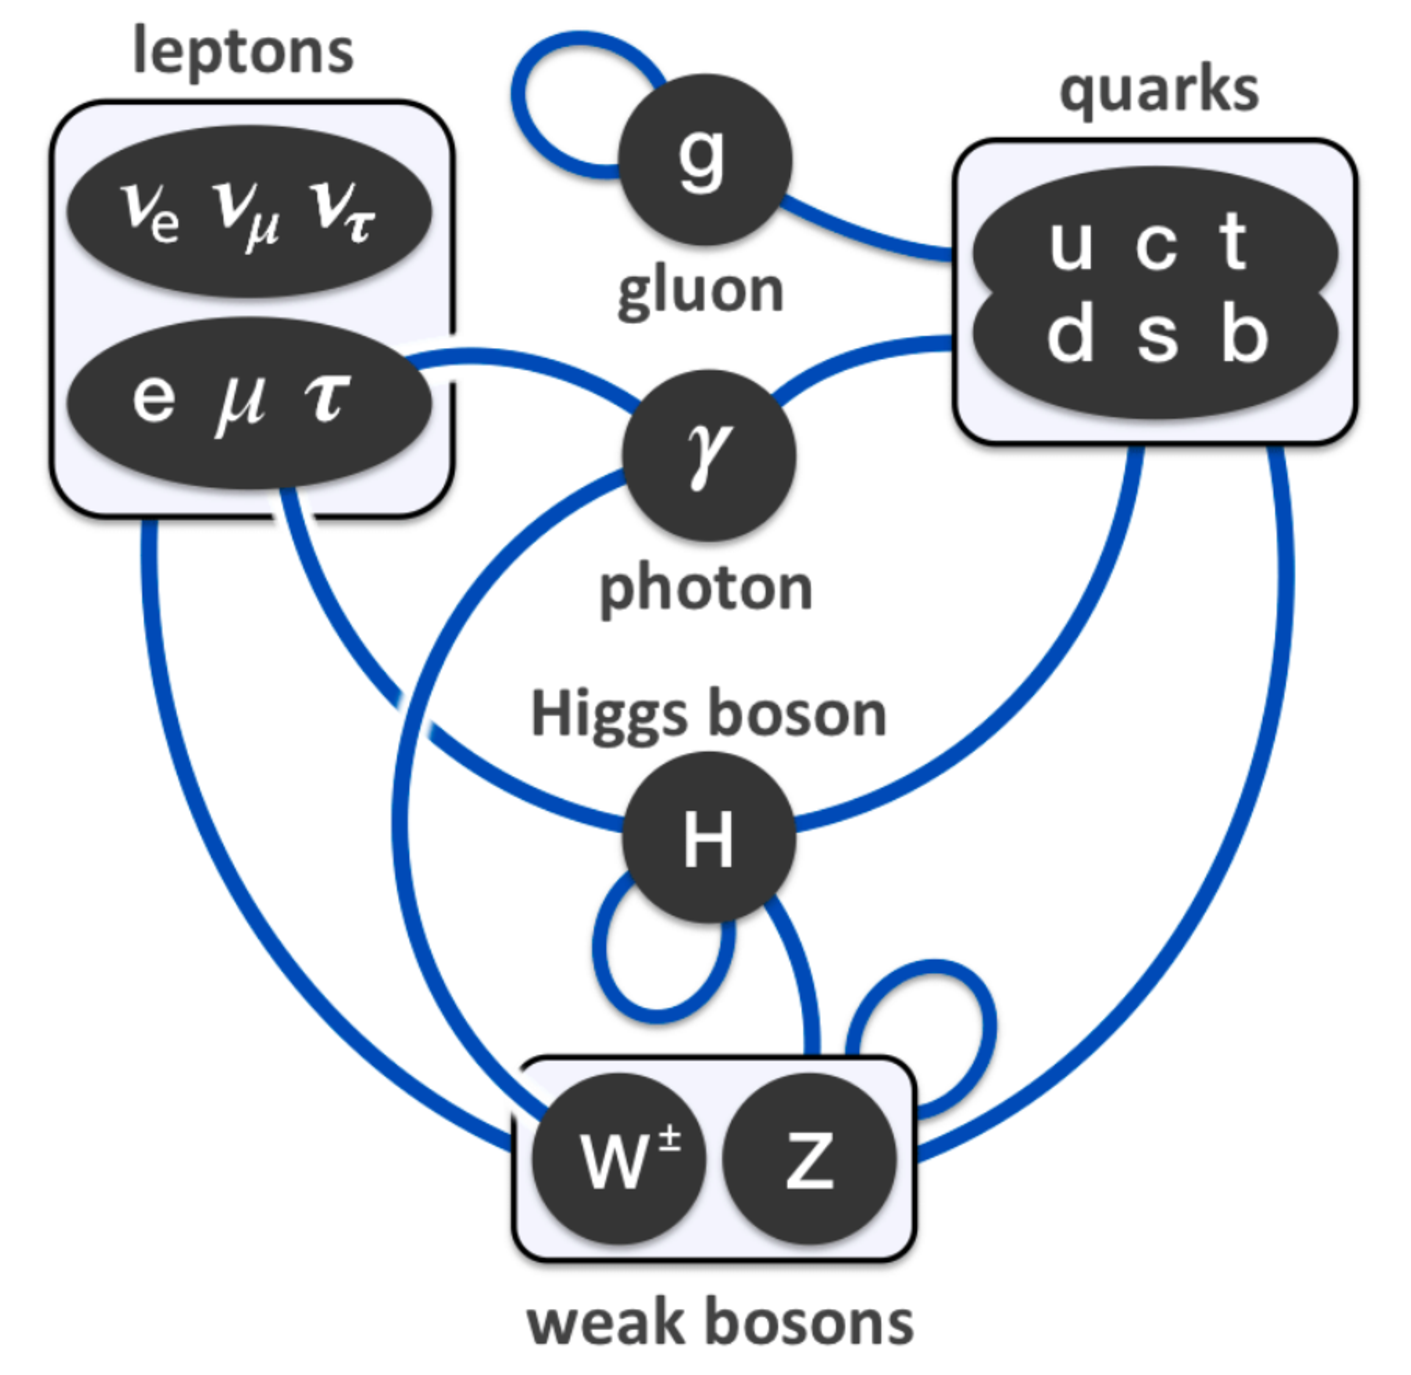
\includegraphics[width=0.5\linewidth]{figures/SMpic.pdf} 
   \caption[Overview of the Standard Model.]{The Standard Model with its fermions and bosons and the involved interactions. The solid blue line indicates which particles interact with each other. Loops depict self-interaction. \cite{SMpic}}
  \label{SMpic}                                     
 \end{center}
\end{figure}
%
Figure \ref{SMpic} summarizes the picture of the SM with its fermions and bosons. The lines indicate which particles interact with each other through the mediators, including self-interaction.
%Gedanken zum SM
%strong (n und p of same duplet) and weak isospin (chirality)
%%%%%%%%%%%%%%%%%%%%%%%%%%%%%%%%%%%%%%%%%%%%%%%%%%%%%%%%%%%%%%%%%%%%%%%%%%%%%%%%%%%%%%%%%%%%%%%%%%%%%%%%%%%%%%%%%%%%%%%%%%%%
\section{Beyond the scope of the Standard Model}\label{beyondSM}
Nevertheless there are still many puzzles left which are not described by the SM. That circumstance keeps physicists well motivated to gain further progress and to push the frontiers of our understanding. \cite{Nair}
\paragraph{Neutrino masses} are confirmed by various neutrino oscillation experiments \cite{Kajita}\cite{McDonald}, although the SM does not predict neutrino masses. The neutrino flavor states $\nu_\alpha$ with $\alpha=e,\mu,\tau$ are quantum entangled with the mass states $\nu_i$ where $i=1,2,3$ described by an unitary matrix $U_{\alpha i}$ \cite{mixing}. One possible extension of the SM, explaining neutrino masses, is the seesaw meachanism. Because of the absence of the right chirality spinor components $\Psi_{R,j}$, the mass term of the Dirac lagrangian $\bar{\Psi}_L\Psi_R+\bar{\Psi}_R\Psi_L$ cannot be formed in case of neutrinos. One possible solution is to describe the neutrino masses with a Majorana mass term, which introduces very massive\footnote{So massive that they are beyond the today`s mass limits, because so far there is no experimental evidence for such neutrinos \cite{Nair}.} right-chiral neutrinos besides light weight left-chiral neutrinos. One caveat is that such right-chiral neutrinos then have to exist, although within the SM there are only left-handed neutrinos known. \cite{Nair}
\paragraph{Quantum gravity} could be the embedding of general relativity into a framework of quantum theory. Quantum theory provides a well confirmed framework for all theories describing particular interactions. Therefore it would be appealing to have a quantum formulation of gravity, following the example of all other fundamental forces and being one step closer to an unificated description. From the view point of cosmology, quantum gravity could be an encompassing theory for a more fundamental understanding where general relativity breaks down, when it comes to the initial conditions of the early universe or conditions of black holes. \cite{quantumgravity}
\paragraph{The hierarchy problem} is a current challenge in particle physics and arises from quadratic corrections to the weak scale. \cite{hierarchy} The hierarchy problem formulates the huge differences of scales where symmetries are broken. Considering a single, unifying symmetry, including the standard model symmetries $SU(3)_c\times SU(2)_L\times U(1)_Y$ (see chapter \ref{SM}),which has to be broken at scale $V$, because it is not manifested at the currently explored energy scales. A lower bound is $V\approx 10^{37}\,\text{GeV}$. At the same time spontaneous symmetry breaking takes place for $SU(2)_L\times U(1)_Y$ at scales of $v\approx\SI{246}{\giga\electronvolt}$\footnote{This is the vacuum expectation value for the Higgs field. \cite{VEV}} in order to get massive W$^\pm$ and Z$^0$ bosons as well es massive quarks and leptons. Within the framework of perturbation theory in quantum field theory such great scale differences are difficult to keep due to the fact that corrections of symmetry breaking are controlled by the highest masses involved. The approach for $v$ is $v^2=v_0^2\sum_{i=1}^kc_i\lambda^i V_0^2$ with the initial value $v_0$, the coupling constant $\lambda$ and general coefficients $c_i$. This shows that including the first correction order the equation is $v^2=v_0^2+c_1\lambda V_0^2$. The consequence is that $v_0^2$ has to be adjusted in such a way that it cancels out several decimal places, for instance 25, of the term $c_1\lambda V_0^2$, but the decimal places beyond that limit should add up to the scale of $\SI{246}{\giga\electronvolt}$. This fine tuning is an unsatisfactory situation, even worsened by adding one more order of quantum correction. \cite{Nair} A non-perturbative solution to the hierarchy problem is proposed by supersymmetric models. \cite{nonperturbative} 
%passt hier wahrscheinlich doch nicht so gut hin, ist ja nicht so wesentlich jetzt für mich... Was ich mir vorstellen könnte ist, dass man das als relativierung zu GUT erklärt, dass auch GUT nicht die eierlegende Wollmilchsau ist--
\paragraph{Supersymmmetry (SUSY)} is a symmetry, which unifies fermions and bosons. The corresponding transformation can be described with an operator in spinor form $Q_{\alpha i}$ and converts fermion fields into boson fields and vice versa. Here $\alpha$ is the spinor index and $i$ are internal degrees of freedom. The field pairs are called superpartners (sparticles) and belong to the same multiplet. The difference between particles and sparticles is the spin quantum number which distinguishes them by half an unit of $\hbar$. \cite{Vergados} Due to no evidence of sparticles, having masses in the same range as the already known elementary particles, also supersymmetry has to be broken. \cite{PhysTeV}. {\SUSY} is very attractive, because it can solve the hierarchy problem, achieve gauge unification and can even provide a candidate for dark matter. \cite{Nagashima} There are two main categories of supersymmetry models, namely $R$-parity conserving and $R$-parity violating models. $R$ is a discrete symmetry in the coupling of particles and their superpartners, defined as \cite{Vergados}:
\begin{align}
                        R=(-1)^{2S+3B+L}=                                       \begin{cases}
                                        +1 & \, \text{for ordinary particles} \\
                                        -1 & \, \text{for {\SUSY} particles}     \end{cases}
                                        \text{,}
\label{Rparity}
\end{align}
where $S$ is the spin, $B$ the baryon number and $L$ the lepton number. An exactly conserved $R$-parity will result in a stable lightest supersymmetric particle and the {\SUSY} particles will be produced in pairs. Whereas a $R$-parity violation will result in singly producable sparticles and all of them are intrinsically unstable. \cite{Kuze}
%%%%%%%%%%%%%%%%%%%%%%%%%%%%%%%%%%%%%%%%%%%%%%%%%%%%%%%%%%%%%%%%%%%%%%%%%%%%%%%%%%%%%%%%%%%%%%%%%%%%%%%%%%%%%%%%%%%%%%%%%%%%
\section{Leptoquarks}\label{LQmodels}
Different shortcomings of the Standardmodel open up chances to extend the the current understanding with concepts briefly introduced in chapter \ref{beyondSM}. One basic idea further develops the symmetry approach, taking the current one as an example (see chapter \ref{SM}), into a great unified theory ({\GUT}). This can be made possible by embedding the SM gauge groups $SU(3)_c\times SU(2)_L\times U(1)_Y$ into a higher symmetry $G_\text{{\GUT}}$. This group has to be broken at the so called ${\GUT}$-scale of $\geq 10^{16}\,\SI{}{\giga\electronvolt}$ to such an extend that the three SM interactions occur as seperate interactions. \cite{PhysTeV} The previously mentioned issues in chapter \ref{beyondSM} already gave a hint on this unification concept in different degrees of manifestations and show that {\GUT} is a solution candidate for different issues. Moreover {\GUT}s imply new gauge bosons called leptoquarks (LQ), which would explain the strong similarities between leptons and quarks. \cite{Nagashima}
%
%
\subsection{Leptoquarks and grand unified theories}
The first {\GUT} was proposed by Georgi and Glashow \cite{GeorgiGlashow}. They proposed that the group $SU(5)$ incorporates all the fermions into one multiplet following the same universal coupling. This enables the possibility to transforms leptons and quarks into each other with leptoquarks as mediators. \cite{Perkins} Altought the Georgi-Glashow model had a great impact, this model is ruled out. It predicts a lifetime of the proton of $10^{30}\,\text{y}$, but the current experimental lower limit is $10^{33}\,\text{y}$. \cite{Griffiths}\par%vllt noch einen Feynmangraph zum Proton Zerfall S. 408, Griffiths
Another unifying group would be $SO(10)$, which is broken to $SO(10)\rightarrow SU(4)_c\times SU(2)_L\times SU(2)_R$, where the leptons are treated as a forth color. \cite{PatiSalamExplanation} This model is the Pati-Salam {\GUT} model \cite{PatiSalam}. Here also the right-handed leptons are included, acting different than their left-chiral counterpart as it is expected for solutions of the neutrino masses for example. \cite{PatiSalamExplanation}\par
Other symmetry groups like $E_6$, inspired by superstring models, are also canditates for a {\GUT} theory. \cite{E6} $E_6$ has a rank of $6$ and is member of the exceptional Lie groups. Furthermore it can be seen as the natural extension of $SU(5)$ and $SU(10)$ and includes a greater set of particles, interpreting them as dark matter candidates. \cite{E6explanation}
%
%
\subsection{Effective Leptoquark models}\label{effmodels}
%12 new mediators X (charge +-4/3, 3 colors = 6) und Y (charge +-1/3, 3 colors = 6) they couple to anti quarks and leptons (anti d liegt  im selben multiplet wie e-) griffiths
%X(Q,I3,Y)=(4/3,1/2,5/3), >(Q,I3,Y)=(1/3,-1/2,5/3) Nagashima
%gauge bosons both with su3 and su2 quantum numbers. these are associated with generators E_ar^+ a =1,2,3 r=4,5- These will be indicated as (X_mu)^alpha and (Y_mu)^alpha associated with r = 4,5 respectively. They occupy the positions indicated by alpha and r. the gauge bosons associated with E_alphar^- are the adjoined of the above and will be indicated as (X_mu)_alpha and (Y_mu)_alpha or equivalently as (Xbar_mu)^alpha and (Ybar_mu)^alpha. the gauge bosons X und Y are triplets under su3 and doublets under su2 and have hypercharge xxx and xxx (wie bei griffiths) vergados
%The known fermions split into three generations each containing 15 states. for example the first generation comprises u and d each in three colors and helicity states, the e- in two helicity states and the nu_e with one helicity state. by convention su5 multiplets are written down as LH states and  RH states are replaced by LH antiparticles (since CP symmetry e-_Land e+_L are equivalent, the RH states of course appear in seperate multiplets) Perkins
\begin{table}[htbp]
		\centering
                \renewcommand{\arraystretch}{1.2}       
		\begin{tabular*}{\linewidth}{@{\extracolsep{\fill}}cccc|cccc}
		\hline
		\hline
		\multicolumn{4}{c|}{$|F|=2$ leptoquarks}&  \multicolumn{4}{c}{$|F|=0$ leptoquarks}     
		\\
		\hline
		LQ       &       $Q/e$   & $T_3$   &       decay   &       LQ       &       $Q/e$   & $T_3$   &       decay   
		\\
		\hline
		$S_{0,L}$       &$-1/3$       &$0$     &$l^{-}_{L}u_L$ or $\nu_Ld_L$         &$V_{0,L}$      &$-2/3$     &$0$      &$l^{-}_{L}\bar{d}_R$ or $\nu_L\bar{u}_R$
		\\
                $S_{0,R}$       &             &        &$l^{-}_{R}u_R$                      &$V_{0,R}$      &            &         &$l^{-}_{R}\bar{d}_L$ 
                \\
                \hline
                $\tilde{S}_{0,R}$       &$-4/3$       &$0$     &$l^{-}_{R}d_R$              &$\tilde{V}_{0,L}$      &$-5/3$     &$0$      &$l^{-}_{R}\bar{u}_L$ 
                \\
                \hline
                $S_{1,L}$       &$-4/3$       &$-1$     &$l^{-}_{L}d_L$                     &$V_{1,L}$      &$-5/3$     &$-1$      &$l^{-}_{L}\bar{u}_R$
                \\
                         &$-1/3$       &$0$     &$l^{-}_{L}u_L$ or $\nu_Ld_L$              &              &$-2/3$     &$0$      &$l^{-}_{L}\bar{d}_R$ or $\nu_L\bar{u}_R$
                \\
                        &$2/3$       &$1$     &$\nu_Lu_L$                                &               &$1/3$     &$1$      &$\nu_L\bar{d}_R$
                \\
                \hline
                $V_{1/2,L}$       &$-4/3$       &$-1/2$     &$l^{-}_{L}d_R$                &$S_{1/2,L}$      &$-5/3$     &$-1/2$      &$l^{-}_{L}\bar{u}_L$
                \\
                $V_{1/2,R}$       &$-4/3$       &           &$l^{-}_{R}d_L$                &$S_{1/2,R}$      &$-5/3$    &             &$l^{-}_{R}\bar{u}_R$
                \\
                                &$-1/3$       &$1/2$      &$l^{-}_{R}u_L$                 &               &$-2/3$     &$1/2$      &$l^{-}_{R}\bar{d}_R$
                \\
                \hline
                $\tilde{V}_{1/2,L}$       &$-1/3$       &$-1/2$     &$l^{-}_{L}u_R$        &$\tilde{S}_{1/2,L}$      &$-2/3$     &$-1/2$      &$l^{-}_{L}\bar{d}_L$
                \\
                                &$2/3$       &$1/2$     &$\nu_Lu_R$                     &                &$1/3$     &$1/2$      &$\nu_L\bar{d}_L$
                \\
		\hline
		\hline
		\end{tabular*}
		\caption[Overview of the scalar and vector leptoquarks proposed by the minimal-Buchm\"{u}ller-R\"{u}ckl-Wyler model.]{Overview of the scalar (S) and vector (V) leptoquarks proposed by the minimal-Buchm\"{u}ller-R\"{u}ckl-Wyler model with their third component of the weak isospin $T_3$, electrical charge $Q$ and the fermion number $F$. The fourth column shows possible decays of the leptoquarks. \cite{Kuze}}
\label{LQstable}
\renewcommand{\arraystretch}{1}
\end{table}
%
The introduction of the effective leptoquark models closely follows \cite{Kuze}.\newline
Leptoquarks are color-triplet scalar $(S)$ or vector $(V)$ bosons having baryon and lepton numbers and carry fractional electrical charge. \cite{Kuze} A general formulation of an effective Lagrangian for leptoquark interaction with the SM fermions was proposed by Buchm\"{u}ller, R\"{u}ckl and Wyler \cite{BRW}. It assumes that LQs
\begin{itemize}
\item[(i)] have renormalizable interactions.
\item[(ii)] have interactions invariant under the SM gauge symmetries $SU(3)_c\times SU(2)_L\times U(1)_Y$.
\item[(iii)] couple only to the SM fermions, gauge bosons and the Higgs boson.
\item[(iv)] are required to conserve the lepton number $L$ and the baryon number $B$ seperately. They carry the fermion number
\begin{align}
                        F=3B+L
\label{fermionnumber}
\end{align}
of $|F|=0$ or $|F|=2$.
\item[(v)] each LQ couples to only a single quark-lepton generation, i.e. three LQ families.
\item[(vi)] has pure chiral couplings to the SM fermions.
\end{itemize}
Condition (iv) makes sure that the proton instability is avoided. Condition (v) only allows inter-generational interactions and large tree-level flavor changing neutral currents and flavor universalites. Condition (vi) supresses contributions to chirally meson decays like $\pi\rightarrow e\nu$. The LQ model, fulfilling (i)-(vi), is the so called minimal-Buchm\"{u}ller-R\"{u}ckl-Wyler effective model (mBRW) with coupling constant $\lambda$. \cite{Kuze}\newline
Fourteen different leptoquark types are known and are listed in table \ref{LQstable}. The same symbol represents LQs of different electric charge within an isospin family, i.e. $S_{1/2,L}$ stands for both, the $S_{1/2}$ state of charge $-\frac53$ and for $-\frac23$. Here $l_X$ are the left-handed lepton doublets in case of $X=L$ and the right handed lepton singlet in case of $X=R$. This differentiation between left-chiral and right-chiral is also valid for the quarks $q_X$ of up-type ($q=u$) or down-type ($q=d$). Seven of the fourteen LQs are scalars ($S_{0,L}$, $S_{0,R}$, $\tilde{S}_{0,R}$, $S_{1,L}$, $S_{1/2,L}$, $S_{1/2,R}$, $\tilde{S}_{1/2,L}$) and seven are vectors ($V_{0,L}$, $V_{0,R}$, $\tilde{V}_{0,R}$, $V_{1,L}$, $V_{1/2,L}$, $V_{1/2,R}$, $\tilde{V}_{1/2,L}$) with their fermion number $|F|=0$ and $|F|=2$. For specific models based on mBRW the branching ratio $\beta(LQ\rightarrow lq)$ are usually fixed to values like $0$, $\frac12$ or $1$. \cite{Kuze}\par
From the experimentalist point of view it makes sense to expand the phenomenology of leptoquarks and ease some restrictions of the mBRW model, giving rise to more generic models. One example is to assume the  branching ratio $\beta$ as a free parameter. Relaxing (iv) or (v) in the lepton sector could open new lepton-flavour violating decays. The result is that the search for leptoquarks is more sensitive to all the various possibilities. \cite{Kuze}
%https://edoc.ub.uni-muenchen.de/9100/1/Krobath_Gernot.pdf
%https://arxiv.org/pdf/hep-ph/9709356.pdf
%https://arxiv.org/pdf/hep-ex/0211048.pdf
%https://ac.els-cdn.com/037026938790637X/1-s2.0-037026938790637X-main.pdf?_tid=7fd73e94-a159-4098-a0c1-5df2ae6f102b&acdnat=1542542854_1685c5ae7ed0ff0824a75e01ecf264ea
%https://journals.aps.org/prd/pdf/10.1103/PhysRevD.8.1240
%https://journals.aps.org/prd/pdf/10.1103/PhysRevD.37.3165
%
%
\subsection{Leptoquark-like couplings in supersymmetry}
An additional generic picture can result from the view point of supersymmetry. In $R$-parity violating {\SUSY} models squarks can produce leptoquark-like signature, because of decay modes involving Yukawa coupling\footnote{Yukawa coupling describes the interaction of a scalar field with a scalar or pseudoscalar Dirac field \cite{Peskin}.}. The left-chiral $\tilde{u}_L$\footnote{Usually the supersymmetric partner particles are denoted with a tilde $\left(\widetilde{\quad}\right)$.} squark couples to a $e^++d$ pair similar a leptoquark $\tilde{S}_{1/2,L}$ with electrical charge of $|Q|=\frac23 e$ would do. Analogous the $\tilde{d}_R$ squark couples to a $e^-+u$ pair or $\nu_e+d$ pair and mimics a $S_0$ leptoquark of charge $|Q|=\frac13 e$. From an experimental view point, the oberservation of such decay is not only restricted to LQ models, but also has implications for the coupling constant of a possible {\SUSY} models. \cite{Kuze}     
%
%
\subsection{Leptoquark pair production in proton-proton collisions}\label{LQpp}
For the search of leptoquarks, the mBRW model (see chapter \ref{effmodels}) is taken as basis.\newline 
At proton-proton colliders, like the {\LHC}, the leptoquarks can be be produced in pairs by gluon-fusion and smaller contributions of quark-fusion. These main processes are shown in Feynman graphs in figure \ref{LQpairs}. The upper row describes the gluon initated production and the lower one the quark initiated production. The last Feynman graph (lower right) is proportional to the square of the coupling constant ($\lambda^2$) \cite{hunter}\cite{Hewett}. Cross section calculations for such processes and further details can be found for example in reference \cite{Kramer}.  
%
\begin{figure}[htbp]                                 
 \begin{center}                                       
  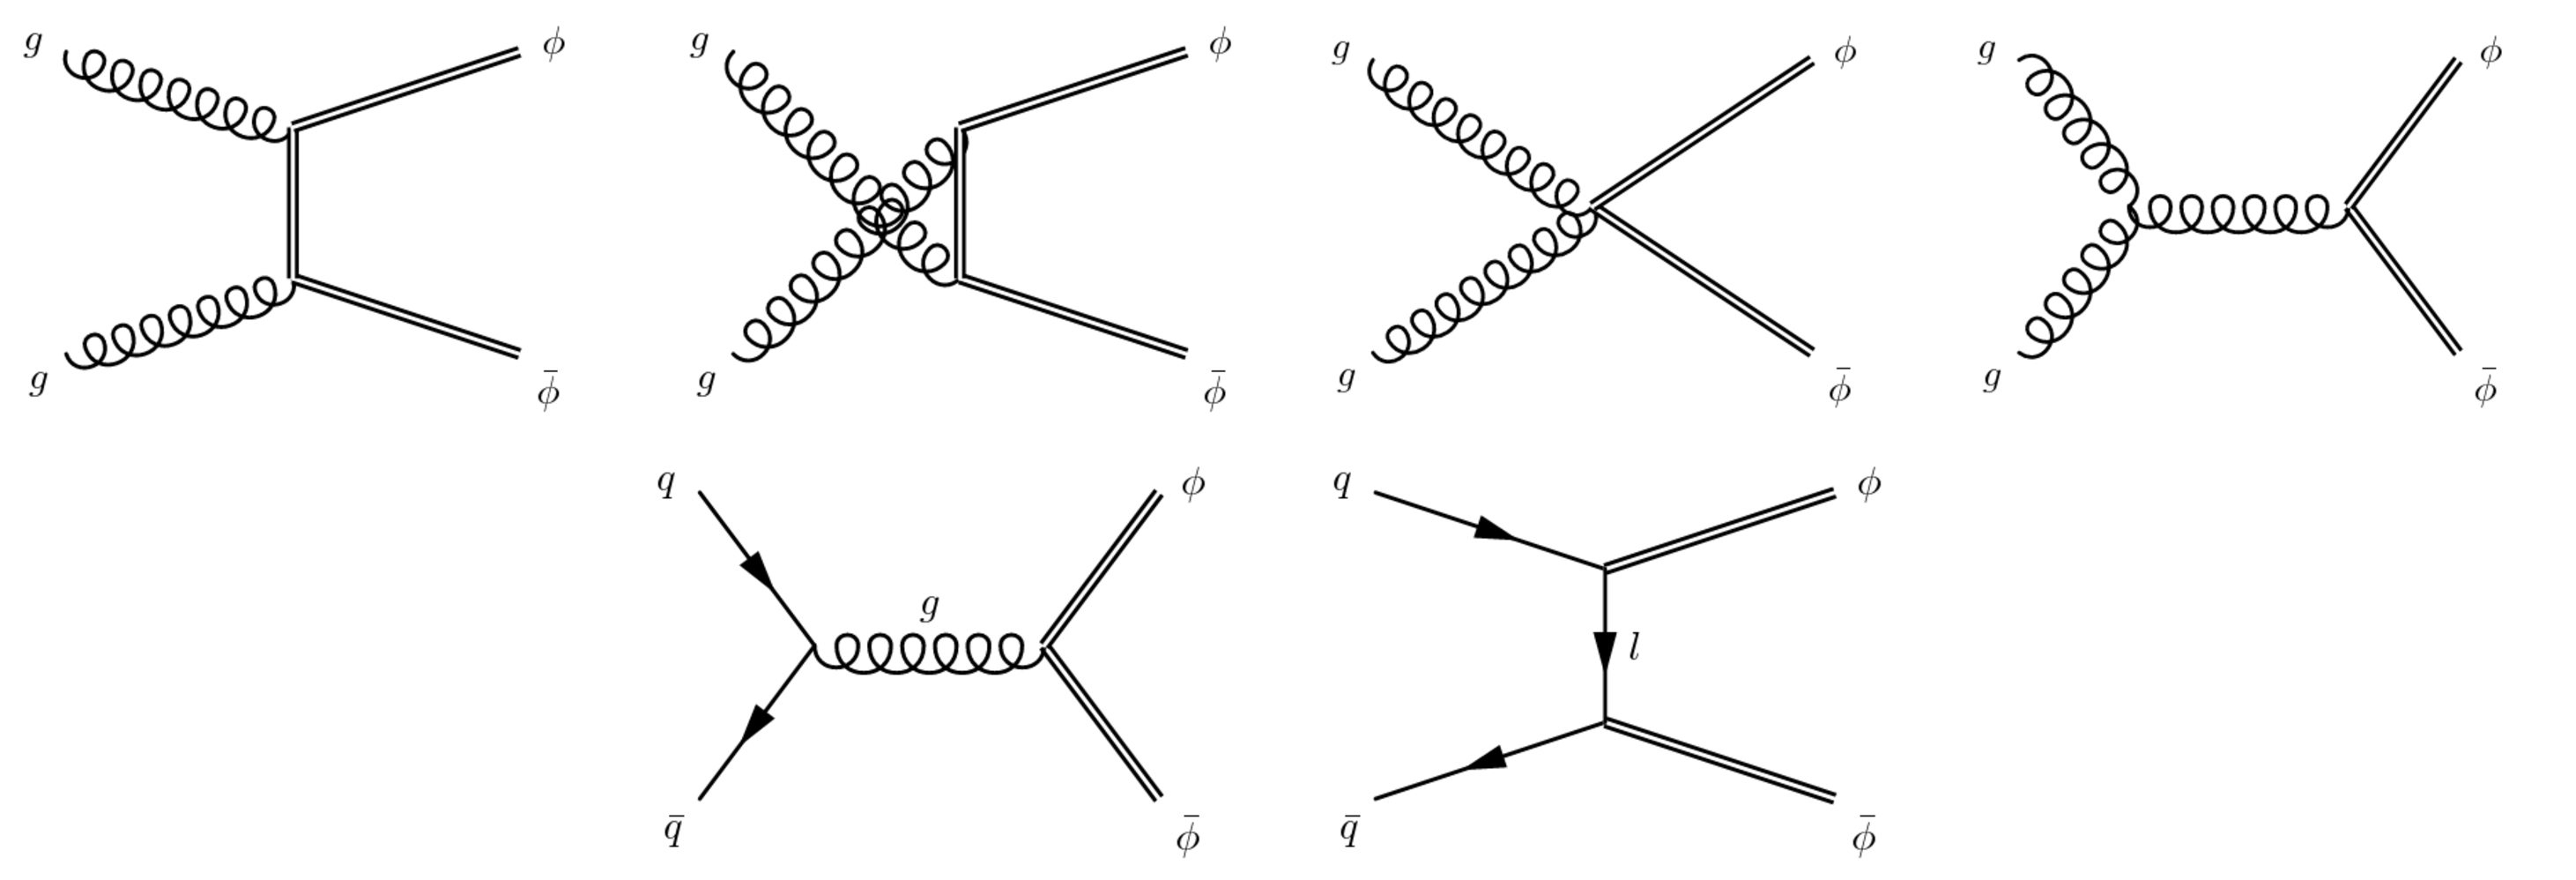
\includegraphics[width=\linewidth]{figures/pairproduction.pdf} 
   \caption[Feynman graphs of leptoquark pair production processes at proton-proton colliders like the {\LHC}.]{Feynman graphs of leptoquark pair production processes dominated by gluon-fusion (upper row) and smaller contributions by quark-fusion (lower row) at proton-proton colliders like the {\LHC}. \cite{hunter}}
  \label{LQpairs}                                     
 \end{center}
\end{figure}
%
The detectable final states, in this case with the {\ATLAS} detector, are governed by the Yukawa coupling $\lambda_{lq}$ of the leptoquark directly on the quark $q$ and lepton $l$ (see figure \ref{YukawaLQ}). The model is defined by two parameters derived from $\lambda_{lq}$: The branching ratio $\beta$ and a coupling constant $\lambda$ are connected to the Yukawa coupling constant like $\lambda_{lq}=\sqrt{\beta}\lambda$ for a charged lepton and like $\lambda_{lq}=\sqrt{1-\beta}\lambda$ for neutrinos. \cite{LQATLAS}\par
%
\begin{figure}[htbp]                                 
 \begin{center}                                       
  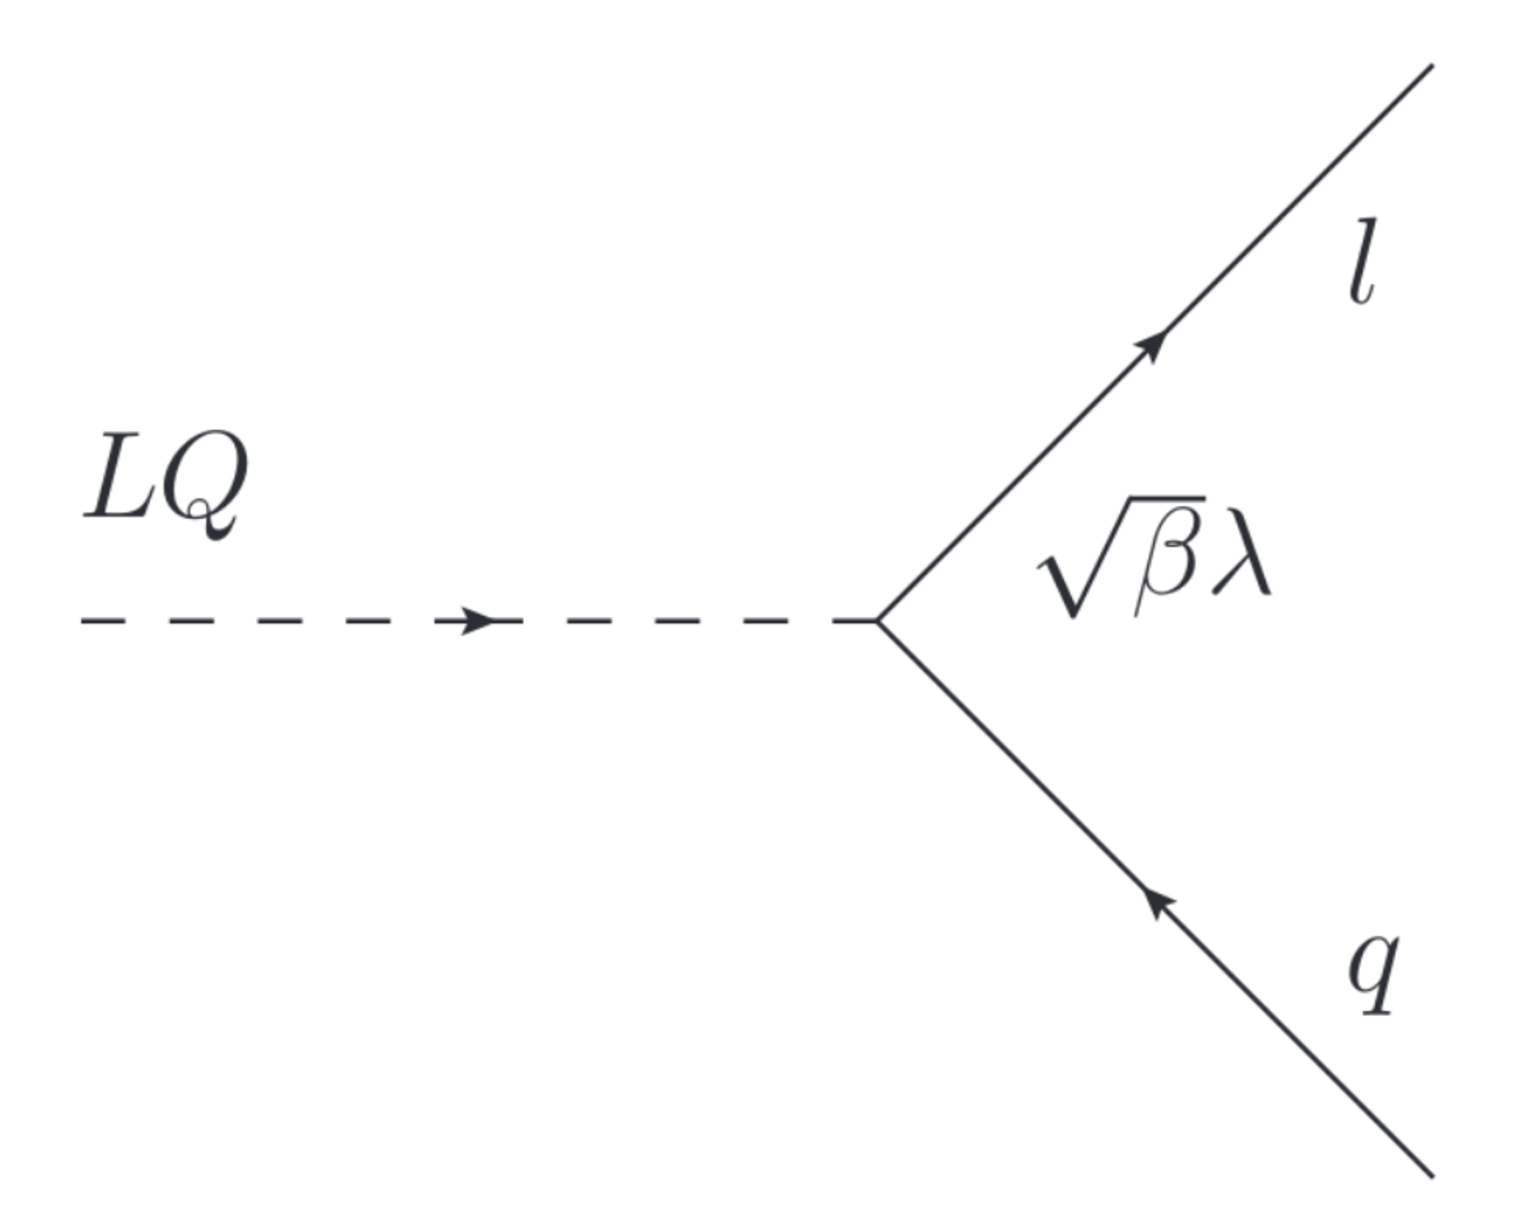
\includegraphics[width=0.444444\linewidth]{figures/yukawa.pdf} 
   \caption[Feynman graphs of a leptoquark decay gouverned by Yukawa coupling.]{Feynman graphs of a leptoquark decay into a lepton $l$ and a quark $q$ gouverned by Yukawa coupling $\lambda_{lq}=\sqrt{\beta}\lambda$. \cite{LQATLAS}}
  \label{YukawaLQ}                                     
 \end{center}
\end{figure}
%
In this thesis the focus lies on the search of pair produced scalar leptoquarks with the final state $LQ+LQ\rightarrow t\tau^{-}+\bar{t}\tau^{+}$. These final states would correspond to leptoquarks $S_{0,L}$ and $S_{1,L}$ (cf. table \ref{LQstable}). \newline
Futher information on the search of vector leptoquarks can be found for example in \cite{vectorLQ} and \cite{vectorLQQ}. 
%https://cds.cern.ch/record/2308307/files/SUgS-18-001-pas.pdf guter Ausgangspunkt auch für LQ Literatur Suche
%%%%%%%%%%%%%%%%%%%%%%%%%%%%%%%%%%%%%%%%%%%%%%%%%%%%%%%%%%%%%%%%%%%%%%%%%%%%%%%%%%%%%%%%%%%%%%%%%%%%%%%%%%%%%%%%%%%%%%%%%%%%%
\chapter{Experimental setup for the search for scalar leptoquarks}\label{experiment}
For the search for scalar leptoquarks the {\ATLAS} detector at the Large Hadron Collider ({\LHC}) is used as experimental setup, which will be described within this chapter. The general setting of the proton-proton collider located at the {\CERN} research center is the topic of section \ref{LHC}. The particle detection of the resulting collision events will take place in the {\ATLAS} detector with its different specialized components (section \ref{ATLAS}). Section \ref{LQpp} addresses the possible leptoquark pair production in proton-proton collisions.  
%%%%%%%%%%%%%%%%%%%%%%%%%%%%%%%%%%%%%%%%%%%%%%%%%%%%%%%%%%%%%%%%%%%%%%%%%%%%%%%%
\section{The Large Hadron Collider accelerator complex}\label{LHC}
The research center {\CERN} (Conseil Europ\'{e}en pour la Recherche Nucl\'{e}aire) was founded in $1954$ near Geneva, Switzerland to become a major European joint venture on elementary particle physics. Currently, $22$ member states are participating in that large-scale project with the ambition to probe the essential constituents of nature and the fundamental forces acting between them. \cite{CERNabout}\par
%
\begin{figure}[htbp]                                 
 \begin{center}                                       
  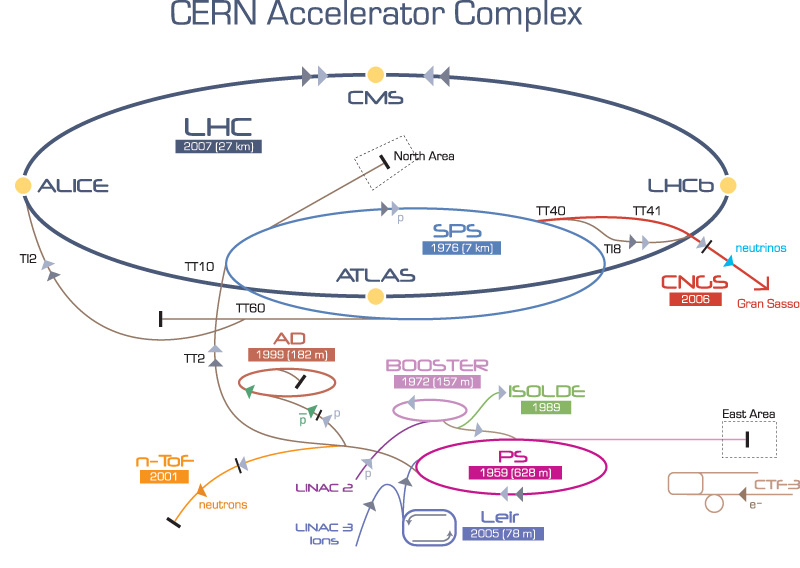
\includegraphics[width=0.8\linewidth]{figures/CERNKomplex2.jpg} 
   \caption[Schematic of the {\CERN} accelerator complex.]{Schematic of the {\CERN} accelerator complex with its different stages and few experiments like {\ATLAS} located at one crossing point for protons. \cite{CERNKomplex}}
  \label{complex}                                     
 \end{center}
\end{figure}
%
In the accelerator complex protons reach energies of $\SI{6.5}{\tera\electronvolt}$ by going through different accelerator stages and are brought to collisions at defined interaction sites in time intervals of $\SI{25}{\nano\second}$. Particle detectors then register signatures of the resulting collision events and the analysis of newly created particles gives insight to the nature of elementary particle physics.\newline 
Figure \ref{complex} shows the different acceleration stages. Starting from the injection, protons will gain a kinetic energy of $\SI{50}{\mega\electronvolt}$ in the linear accelerator {\LINAC}2 and will be further transferred to the Proton Synchrotron Booster ($\SI{1.4}{\giga\electronvolt}$), the Proton Synchrotron ($\SI{25}{\giga\electronvolt}$), the Super Proton Synchrotron ($\SI{450}{\giga\electronvolt}$) and finally to the {\LHC} ring with its $\SI{26.7}{\kilo\meter}$ circumference. \cite{CERNabout}\newline
The {\LHC} is designed as two-ring proton-proton collider. Conditions for a stable proton beam are diverse, including high vacua of $\SI{E-10}{\milli\bar}$ to $\SI{E-11}{\milli\bar}$ and temperatures of $\SI{1.9}{\kelvin}$ for the superconducting NbTi-magnets of the accelerator. \cite{LHCJINST}\par   
%hier dann weiter ins Detail wie LHC JINST #######################
%Die Idee ist eigentlich eine genauere Beschreibung der Komponenten, allerdings ist JINST schon wieder so tief... So überblicksmäßiger wäre viel bessser, bei dem man noch im Blick behalten kann, um was es eigentlich geht...
Different experiments like \ALICE\cite{ALICE}, {{\LHC}}b\cite{LHCb} are located at the {\LHC} due to the variety of research questions. But the subject of interest in this work lies in the high luminosity experiment {\ATLAS}, which is specialized for proton-proton collisions, like its counterpart \CMS\cite{CMS}. Main tasks of {\ATLAS} are more precise measurements of the SM (see chapter \ref{SM}), better understanding Quantum Chromo Dynamics (QCD) and search for supersymmetric models, and new physics, among others. With the {\LHC} production of $10^9$ inelastic events per second, up to $23$ simultaneously events at dominating high QCD cross sections reqiure a powerful detector that is capable of recognizing the characteristic signatures. These circumstances make up the demands for {\ATLAS}, including fast electronic elements, high detector granularity, handling high particles fluxes and reducing overlapping events at a large acceptance and coverage region. \cite{ATLASJINST}       
%AußerdeM: Hinweis auf high Lumi LHC als Art mini-Ausblick in diesem Kapitel https://arxiv.org/pdf/1705.08830.pdf, https://cds.cern.ch/record/1711887/files/ATL-COM-UPGRADE-2014-014.pdf ################
%%%%%%%%%%%%%%%%%%%%%%%%%%%%%%%%%%%%%%%%%%%%%%%%%%%%%%%%%%%%%%%%%%%%%%%%%%%%%%%%%%%%%%%%%%%%%%%%%%%%%
\section{The ATLAS detector at the LHC}\label{ATLAS}
One of the general purpose detector for proton-proton collisions is the {\ATLAS} detector. This $\SI{25}{\meter}$ tall detector is located at one interaction point of the {\LHC} where bunches, consisting of approximately $\SI{E11}{}$ protons, collide at a rate of $\SI{40}{\mega\hertz}$ \cite{ATLASJINST}. The number of particles encountered per time is given by \cite{Perkins}
\begin{align}
                        \dot{N}=\mathcal{L}\sigma
\end{align}
with the cross section $\sigma$ for the present event and the instantantaneous luminosity $\mathcal{L}$. Given a measure for the number of collisions per unit time the instantaneous luminosity can be introduced and is often used as key parameter in collider physics \cite{LHCJINST}.
\begin{align}
                        \mathcal{L}=\frac{N_bn_bf_{\text{rev}}\gamma_r}{4\pi\epsilon_n\beta^*}F
\label{Lumi}
\end{align}
Where $N_b$ is the number of particles per bunch, $n_b$ the number of bunches per beam, $f_{\text{rev}}$ the rotational frequency, $\gamma_r$ the Lorentz factor, $\epsilon_n$ the normalized transverse beam emittance, $\beta^*$ the betatron function at the collision point and $F$ respects the geometric luminosity reduction factor due to the crossing angle at the collision point. The luminosity of {\ATLAS} exceeded the design luminosity of $\mathcal{L}=\SI{2.05E34}{\per\square\centi\meter\per\second}$ by a factor of $2.05$ on the $2^{\text{nd}}$ of November 2017, emphasizing the great success over the years \cite{designLumiExceeded}.\par 
%Erklärung für Lumi auch aus Perkins? ##########
The aspiration to be sensitive to the great variety of particles governed by the fundamental forces (see chapter \ref{SM}) influenced the detector design accordingly. The layered structure reflects the fact that
%Motivation eher sogar von der Seite, wieso so gebaut, wie er ist --> Teilchen detektieren (Verweis auf SM Kaptiel)-> Schichtaufbau-> etc... #######
The basic structure of {\ATLAS} is shown in figure \ref{ATLASandCoordinate} with its different sub-detector systems together with the convention for the used coordinate system.  %Koordinatensystem
%
\begin{figure}
 \centering
  \begin{subfigure}[c]{0.95\textwidth}
   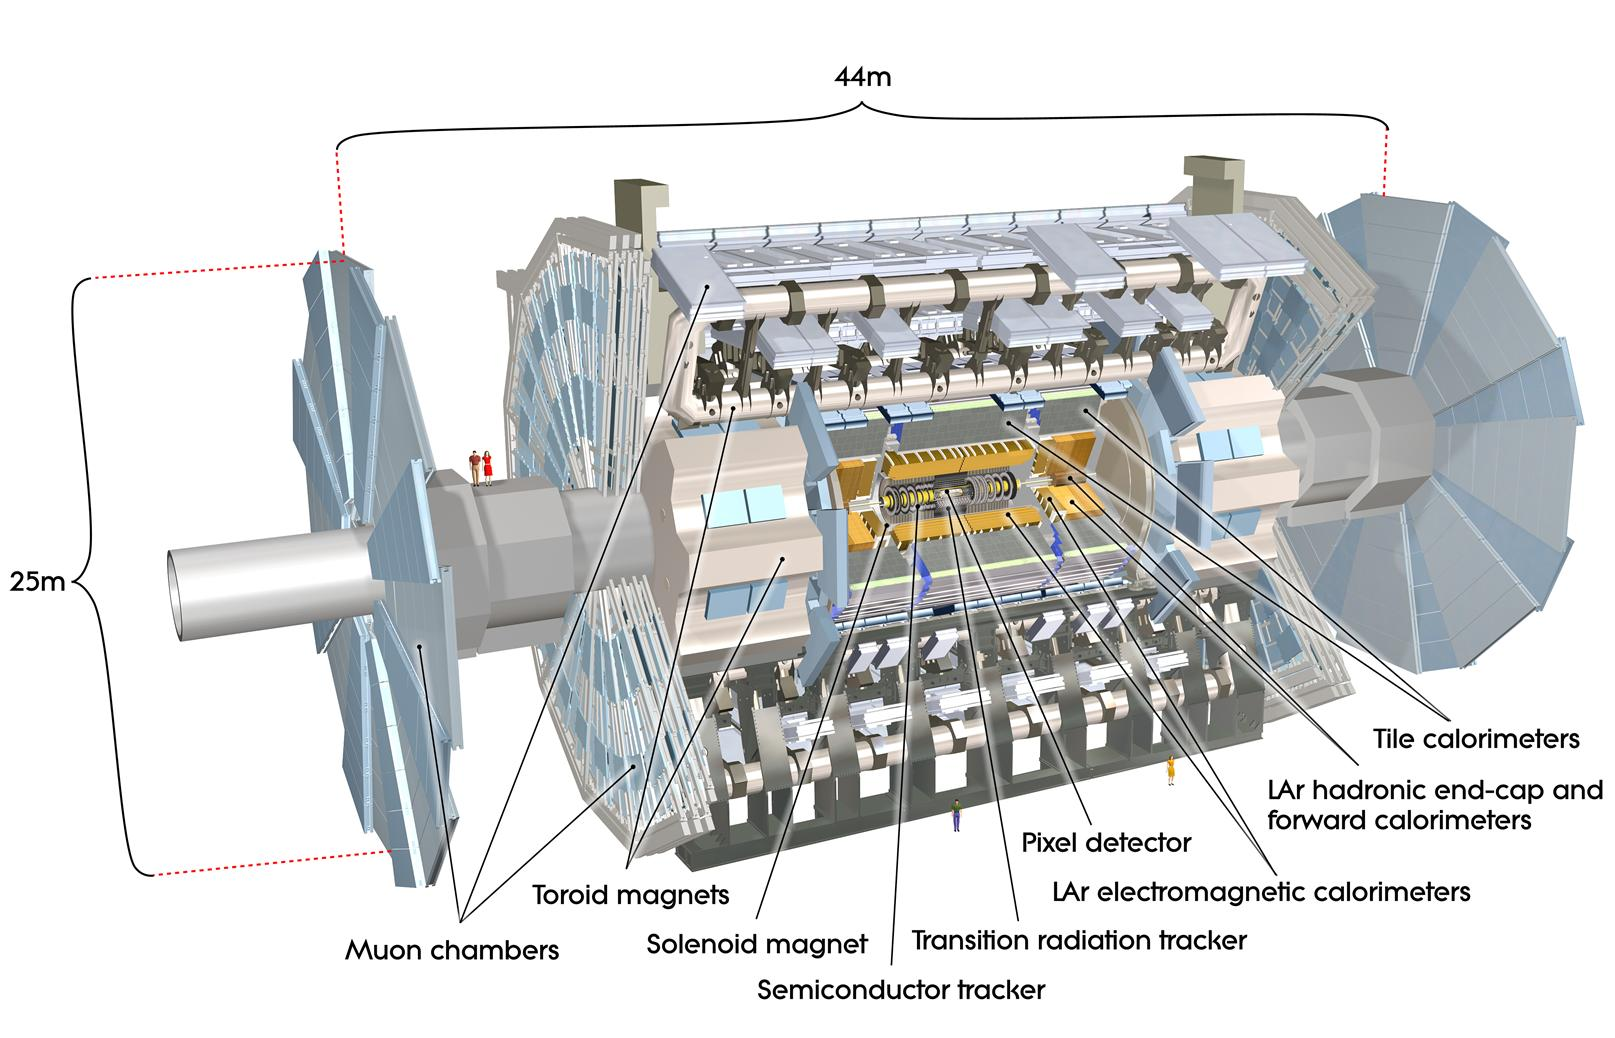
\includegraphics[width=\textwidth]{figures/ATLASDesign.png}
    \subcaption[The structure of the {\ATLAS} detecor and its sub-systems.]{The layered structure of the {\ATLAS} Detector at the {\LHC} with its sub-systems Inner Detector, Calorimeter, magnets and Muon Spectrometer \cite{ATLASJINST}.}
   \label{ATLASDesign}
  \end{subfigure}
  \begin{subfigure}[c]{0.95\textwidth}
   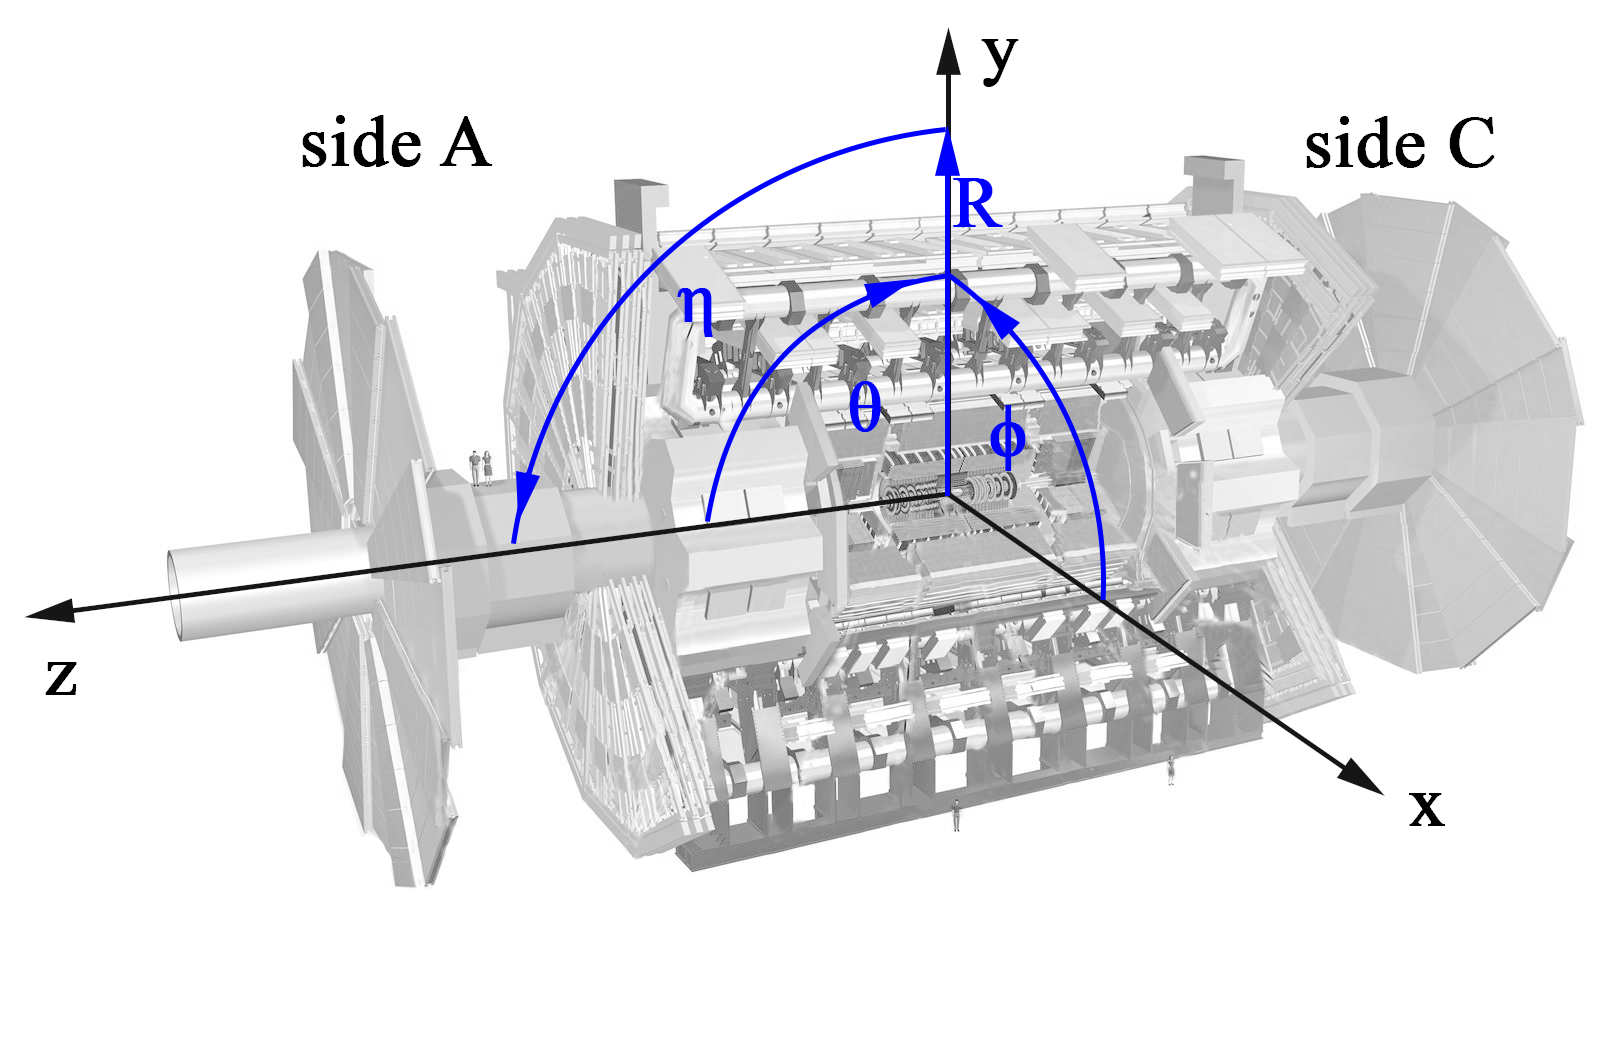
\includegraphics[width=1\textwidth]{figures/ATLASDesignCoordinate.png}
   \subcaption[Definition of the global {\ATLAS} coordinate system.]{The global {\ATLAS} coordinate system formulated in cylindric coordinates with the $z$-axis parallel to the beam line and the transverse plane defined through azimuthal angle $\phi$ and pseudorapidity $\eta$. Based on \cite{ATLASJINST}.}
   \label{Coordinate}
  \end{subfigure}
 \caption[Structure of the {\ATLAS} detector and the used coordinate system.]{Structure of the {\ATLAS} detector and the used coordinate system.}
 \label{ATLASandCoordinate}
\end{figure}
%
The nominal interaction point acts as origin of the coordinate system, where the $z$-axis follows the beam line counterclockwise. Perpendicular to the $z$ axis lies the transverse $x$-$y$-plane usually described through the azimuthal angle $\phi$. The positive $x$-axis points towards the center of the {\LHC}. The cylindric symmetry of the detector suggests a cylindric coordinate system with the angle $\theta$ starting from the beamline. \cite{ATLASJINST} Since the polar angle is not a Lorentz invariant quantity, it is useful to describe the position in terms of rapidity \cite{LHCJINST} $w=\frac12\ln{\frac{E+p_zc}{E-p_zc}}$ in that highly relativistic regime. In the limit of large momenta, i.e. $|\mathbf{p}|c\approx E$, the rapidity coincides with the pseudorapidity formulated as \cite{ChinaPseudorapidityBook}
\begin{align}
                        \eta=-\ln{\tan\frac{\theta}{2}}\text{.}
\label{pseudorapidity}
\end{align}
This variable has only the polar angle as dependence and is therefore the adequate quantity in the context of collision experiments, where usually the angle $\theta$ from the beamline is measured. \cite{ChinaPseudorapidityBook}\par      
%Aufbau Idee: auch so ein Walkthrough durch die einzelnen Komponenten wie bei der Bachelorarbeit
%einzelne Komponenten + Trigger(ref auf Datenauswertung, Software part im Text dann)
\textbf{The magnet configuration} includes a superconducting solenoid with a field strength of $\SI{2}{\tesla}$ sourrounding the inner detector as well as three large superconducting toroid magnets composed in an eight-fold azimuthal symmetry around the calorimeter. The barrel toroid magnet delivers a field strength of $\SI{0.5}{\tesla}$ and in the end-cap a field of $\SI{1}{\tesla}$ is present. \cite{ATLASJINST}\newline%Bending particle path -->identification... ######
\textbf{The inner detector} is responsible for pattern recognition, momentum and vertex measurements and electrically charged particle identification which is achieved with a combination of semiconductor pixel and microstrip trackers (SCT). The Insertable B-Layer (IBL) is the innermost layer of the pixel detectors at a radius of $\SI{3.3}{\centi\meter}$ away from the beam line. Additional straw tube tracking detectors are sensitive to transistion radiation (TRT) in the outer part that are responsible for high vertex and momentum resolution. The $R-\phi$ segmented pixel detectors are of size $50\times \SI{400}{\square\micro\meter}$ and the SCTs with its $8$ strip layers cover together a range of $|\eta|<2.5$. Typically $36$ hits per track are provided by the $\SI{4}{\milli\meter}$ straw tubes of the TRTs, which cover the range $|\eta|\leq 2.0$. \cite{IBL}\cite{ATLASJINST}\newline %Unterscheidung teilchen anhand der Übergangsstrahlung ####################
Liquid argon electromagnetic sampling \textbf{calorimeters} with high granularity allow an excellent energy measurement for electrons and photons. It has a total thickness of more than $22$ radiation lengths $X_0$ in the barrel region ($|\eta|<1.475$) and more than $24X_0$ in the end-cap region ($1.375<|\eta|<3.2$). For hadronic energy measurements a scintillator-tile calorimeter covering $|\eta|<1.7$ is in operation. It is a sampling calorimeter and uses steel as absorber material and scintillating tiles as active material in conjunction with wavelength shifting fibres. Further LAr technology is used for hadronic particles in the outer pseudorapidity range up to $|\eta|=3.2$. Here copper plates provide the absorber material. The forward calorimeters extend the coverage for hadronic and electromagnetic energy measurements to $|\eta|=4.9$ and are $10X_0$ deep. \cite{ATLASJINST}\newline%Energiemessung: provide god res for high energy jets###################
The \textbf{muon system} is suited in the outer layer of {\ATLAS} and provides as independent system resolution for high energy muon tracks with three layered precision chambers. This is possible because of the air-cored toroid magnet system including one barrel and two end-cap magnets generating strong bending power in a large volume and delivering  a mostly perpendicular magnetic field regarding the muon trajectories. The bending power $\int{\vec{B}d\vec{l}}$ along the track of the muon $d\vec{l}$ reaches $\SI{1.5}{\tesla\meter}$ to $\SI{5.5}{\tesla\meter}$ in the range $|\eta|<1.4$ (barrel) and up to $\SI{7.5}{\tesla\meter}$ (end-cap). The precision chambers are Monitored Drift Tubes (MDT) and in the larger pseudorapidity range Chathode Strip Chambers (CSC) which are multiwire proportional chambers. Due to the fact that the overall performance depends crucially on the alignment of the muon detectors with respect to each other and in respect to the Inner Detector, MDTs are equipped with a optical monitoring system with $1200$ sensors. Resistive Plate Chambers (RPC) and Thin Gap Chambers (TGC) are the constituents of the muon trigger system. \cite{ATLASJINST} \newline %Myonen kommen überall durch-->hier detektieren + Problem der Spurkrümmung für high pt--> eigenes system für die genauere myon-messung ############
Due to technology and resource limitations the data recording rate has to be reduced from $\SI{40}{\mega\hertz}$ to $\SI{200}{\hertz}$. This poses high demands on an efficient \textbf{trigger system} which is organised in three levels. Level $1$ uses only a subset of the total detector information making basic decisions to flag so called regions of interest, i.e. coordinate regions. Searches include patterns for high transverse momenta of muon tracks, electrons and photons as well as jets or large missing energy balances. The output rate after this first selection accounts for $\SI{75}{\kilo\hertz}$. The high level trigger $2$ and $3$ are responsible for selecting the level $1$ triggerd regions at full granularity and precision. The level $3$ event filter is the final stage and achieves data reduction down to the final data-taking rate of $\SI{200}{\hertz}$, writing events of the size of approximately $\SI{1.3}{\mega\byte}$ to the disks. The event filter's selection criteria are implemented using offline analysis procedures. \cite{ATLASJINST}%efficient triggering with sufficient background rejection ##############
%evtl doch das fettgedruckte als einzelne Unterpunkte und dann etwas ausführlicher. Allerdings wird das dann ganz schön lang...
%%%%%%%%%%%%%%%%%%%%%%%%%%%%%%%%%%%%%%%%%%%%%%%%%%%%%%%%%%%%%%%%%%%%%%%%%%%%%%%%%%%%%%%%%%%%%%%%%%%%%%%%
\chapter{Turning detector signatures into physical objects}
All components of the detector system of {\ATLAS} (see chapter \ref{ATLAS}) deliver electronic signals of the proton-proton collisions, which have to be reconstructed to physical objects for the analysis. This chapter describes the reconstruction of the physical objects like electrons, muons, jets and b-flavor jets and taus, which are important for the analysis in this thesis. Furthermore the role of Monte Carlo simulations in the analysis are presented briefly.
%e,l,tau, jet vor bjet natürlich + MC chapter
%
%
\section{Electron reconstruction at ATLAS-- identifying electrons}
Electrons and positrons\footnote{In this section, the term positron is absorbed in the term electron.} give rise to tracks in the Inner Detector of {\ATLAS} and deposit energy in the electromagnetic calorimeter. The tracks and calorimeter signals are used in combination for the electron reconstruction. \cite{ePerformance}\par
For the reconstruction of electrons in the central region ($|\eta|<\SI{2.47}{}$) several steps are needed. At first, respecting the granularity of the calorimeter, it is searched for electron cluster seeds in do called step of \textit{seed-cluster reconstruction}. The efficiency of this search is $\SI{95}{\percent}$ to $\SI{99}{\percent}$ for transverse energies of $\SI{7}{\giga\electronvolt}$ and $>\SI{15}{\giga\electronvolt}$ respectively. The \textit{track reconstruction} is responsible for the pattern recogniztion respecting the energy loss due to mainly bremsstrahlung in the detector material up to $\SI{30}{\percent}$. The track seed, consisting of three hits in different layers of the silicon detectors, is extended to the full track of at least seven hits to the region of interest  at the electromagnetic calorimeter. This is done by the {\ATLAS} Global $\chi^2$ Track Fitter \cite{trackfitter}. Afterwards the matching of the track to a specific cluster in the electromagnetic calorimeter is done in the \textit{electron specific track fit}. The final step, \textit{electron candidate reconstruction}, is the matching of the track candidate to the initial cluster seed. \cite{ePerformance}\newline
Both, the information of the track and the energy cluster, are used for the four-momentum calculation of the electrons. Algorithms for reconstructed electron identification are applied to distinguish signal-like or background-like electron candidates. For that the TRT likelihood method plays an important role, which uses the high-threshold hits of each TRT. Several discriminating variables are evaluated\footnote{For further details see \cite{ePerformance}} for this likelihood method (LH). Based on the outcome, three operating points for the electron identification are defined: \textit{Loose} relies on information of the hadronic calorimeter and the first two layers of the electromagetic calorimeter. \textit{Medium} adds information from the TRTs, the transverse impact parameter and the third layer of the electromagnetic calorimeter, whereas the \textit{Tight} operting point additionally considers track-cluster matching variables. \cite{ePerformance}\newline
For a well reconstructed electron also requirements on the isolation of the cluster and the track are necessary. In this thesis the definition of the operating point \textit{Gradient} is relevant. The efficiency linarly depends on the transverse energy $E_T$. For Gradient the isolation in the calorimeter and the track is $\SI{0.1143}{\percent}\cdot E_T+\SI{92.14}{\percent}$. \cite{ePerformance}
%
%
\section{Muon reconstruction at ATLAS -- identifying muons}
Muons\footnote{In this section, the term anti-muon is absorbed in the term muon.} are reconstructed independently in the inner detector and the muon spectrometer and the resulting combination of the two gives the full muon track. \cite{muPerformance}\par
The first step is again pattern recognition for seeds in the silicon layers from the inside towards the outside of the inner detector. Seeds are formed of three space points. The space points are provided from the pixel detectors with their local two-dimensional space points and from the combination of a pair of SCTs. The default setting of the seeding algorithm allows three combinations for space points: all space points in the pixel detector, all in the SCTs or two in the pixel detector and one in the SCT. \cite{muInner}\newline
The muon reconstruction in the muon spectrometer is initiated by the search of hit patterns in the muon chambers to form segments. Muon track candidates are created by fitting together from the segments in different layers, which is done by an combinatorial search. Selecting criteria include hit multiplicity and fit quality to find the optimal track. The hits associated with each track candidate, after applying an overlap removal algorithm, is fitted using a global $\chi^2$ fit. \cite{muPerformance}\newline
The combination of the muon reconstruction depends on what information of the muon candidate is available in the inner detector and the muon spectrometer. A \textit{combined muon} is reconstructed of the independent inner detector and muon spectrometer measurement in a global refit. \textit{Segment-tagged muons} are extrapolated from the inner detector muon track to at least one local segment of the muon spectrometer. If the track of the inner detector can be matched to energy deposit in the calorimeter, the reconstructed muon is called \textit{calorimeter-tagged} muon. Muons reconstructed only on the basis of the muon spectrometer are extrapolated back to the interaction point and therefore are called \textit{extrapolated muons}.\cite{muPerformance}\newline
Quality requirements on the muon supress background contributions and garantee a robust momentum measurement and include discriminating variables like the $\chi^2$ of the combined track. This categorization finalizes the muon identification process. For the category \textit{Loose muons} all above listed muon types are used. The category \textit{medium muons} minimizes the systematic uncertainties and is based only on combined muons and extrapolated muons. \textit{Tight muons} only uses the combined muon type and is optimized for maximum purity at the cost of some efficiency. The \textit{high-$p_T$ muons} are designed for  a maximazation of the momentum resolution for tracks above $\SI{100}{\giga\electronvolt}$. \cite{muPerformance}\newline
The relevant isolation requirement for this thesis on muons is the so called \textit{Gradient} isolation, which inlcudes track-based and calormieter-based discriminating variables. In this case it is the sum of transverse momenta of the tracks in a cone around the muon with $\Delta R=\sqrt{\Delta\eta^2+\Delta\phi^2}<0.3$, excluding the muon track itself. The calorimeter condition is based on the sum of transverse energies of the topological clusters around the muon in a cone of $\Delta R<0.2$. \cite{muPerformance}\cite{varcone}     
%
%

\section{Jet reconstruction at ATLAS -- identifying jets}\label{jets}
For the reconstructin of hadronic part of final states like isolated hadrons, jets (see also section \ref{btagging}) and hadronically decaying taus (see also section \ref{taus}), the {\ATLAS} experiment employs clusters of topological connected calorimeter cell signals (topo-clusters). The topo-cluster algorithm analyzes the spatial distribution of the cell signals to reconstruct the energy and direction of the incoming particle. \cite{topo}\par
The segmented lateral readout of the highly granularity calorimeter allows the distinction between signals from particle showers and background events by the reference of the cell signal significance $\zeta_\text{cell}^\text{EM}$. \cite{topo} Seeds are defined by cells, where the absolut energy $|E|$ exceeds the noise level by a factor of four standard deviations. The topo-clusters are expanded by iteratively all neighbour cells with energies two standard deviations above the noise level. \cite{jetPerformance}\newline
For this thesis the relevant clustering algorithm is the anti-$k_t$ algorithm. The algorithm needs the following definitions \cite{antikt}:
\begin{align}
                        &d_{ij}=min(k_{ti}^{-2},k_{tj}^{-2})\frac{\Delta_{ij}^2}{R^2}\\
                        &d_{iB}=k_{ti}^{-2}\,\text{,}
\label{antiktalgorithm}
\end{align}
where $d_{ij}$ is the distance between the particles $i$ and $j$ and $d_{iB}$ the distance between $i$ and the beam $B$. $k_t$ denotes the transverse momentum, $R$ is the radius parameter and $\Delta_{ij}^2=(\eta_i-\eta_j)^2+(\phi_i-\phi_j)^2$ denotes the cone between $i$ and $j$. The final clustered jet is achieved with the search of the minimum in distances $d_{iB}$ and $d_{ij}$. If the mimimum is $d_{ij}$, then the sum of the four-momentum of object $i$ and $j$ is calculated and is treated as a new object. Again all distinces between the objects are re-calculated until $d_{iB}$ is a minimum. This is means, object $i$ is the final jet. The anti-$k_t$ algorithm is a stable jet reconstruction algorithm and is not prone to fluctuations due to adding low $k_t$-objects. \cite{antikt}
%
%
\section{b-tagging at ALTAS -- identifying b-jets}\label{btagging}
The third generation quarks, i.e. top (t) and bottom (b), play a crucial role in the SM and its various extension possibilities like the Leptoquark Model due to their large masses \cite{Hansson}. Therefore, it is essential to identify hadrons containing b quarks and seperating them from light-flavour quarks at hadron collider detectors like {\ATLAS}. This task is commonly reffered as b-tagging and can be seen as a classification problem with the goal to assign right jet flavours. To that end the particle tracks in the Inner Detector and the jet reconstruction of clusters in the electromagnetic and hadronic calorimeter are discriminating objects. \cite{Paganini}\par
%
\begin{figure}[htbp]                                 
 \begin{center}                                       
  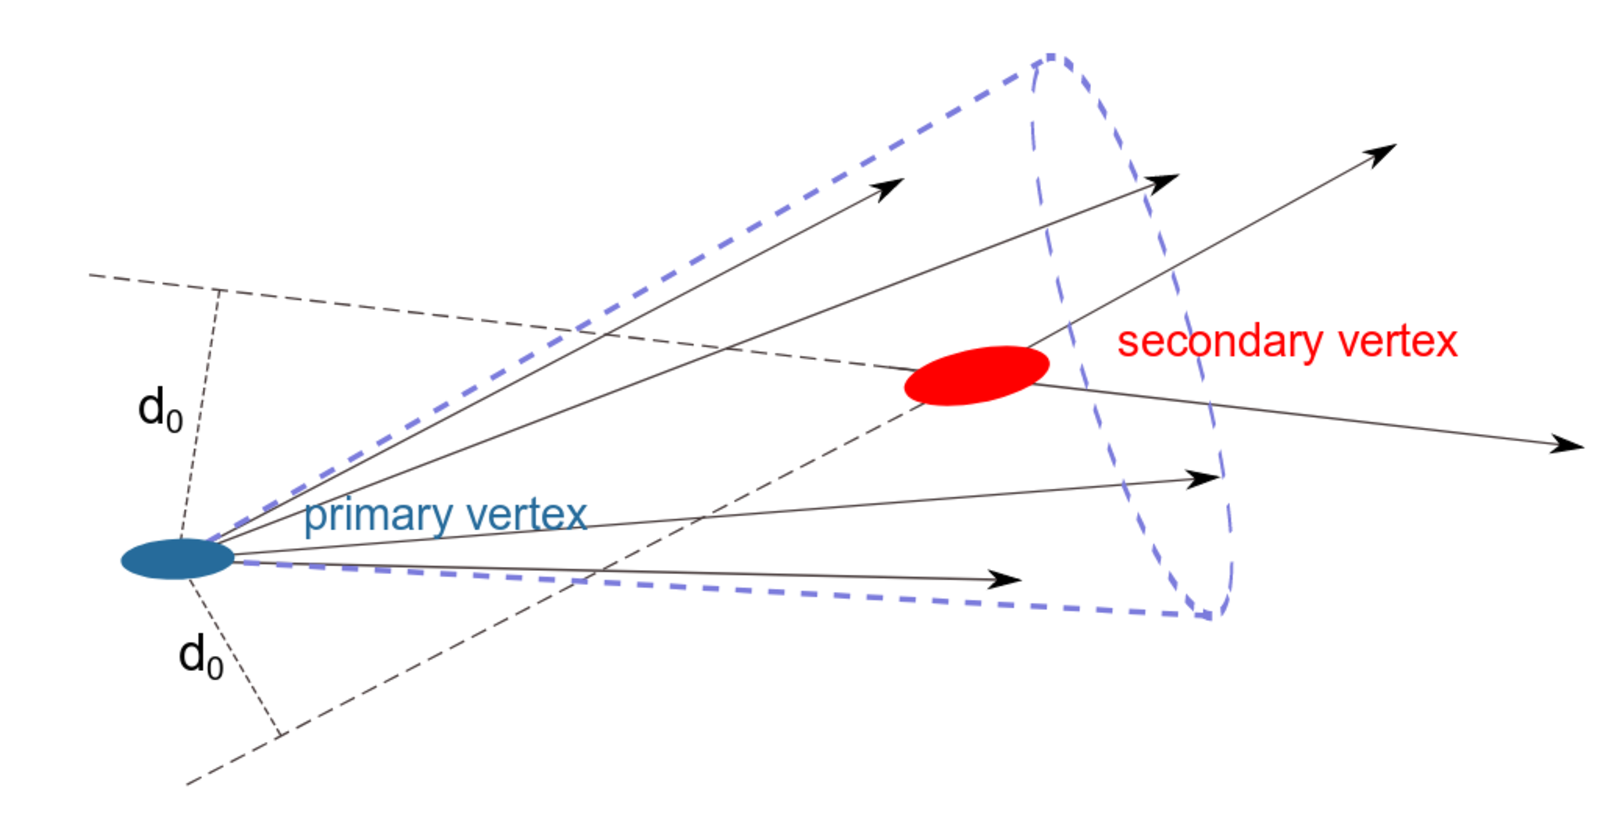
\includegraphics[width=0.55\linewidth]{figures/btagged.pdf} 
   \caption[Tracks in a b-jet.]{Signature of a b-jet with the primary and secondary vertex created relevant for b-tagging. $d_0$ is the impact parameter. \cite{Hansson}}
  \label{btagged}                                    
 \end{center}
\end{figure}
%
The long lifetime of B hadrons in the order of $\SI{1.6}{\pico\second}$ allow them to travel a few millimeters in the detector. The subsequent decay of those heavy particles within a secondary vertex produce tracks with comparably large impact parameter $d_0$ that is the shortest distance of the particle track from the primary vertex (see figure \ref{btagged}). This signature and the deduced impact parameter significance $S(d_0)=\frac{d_o}{\sigma(d_0)}$, where $\sigma(d_0)$ is the uncertainty of the impact parameter, are used by the b-tagging algorithms including five low-level and two high-level taggers. \cite{Hansson} The b-tagging algorithms rely on multivariate combinations of the information and process them to calculate a discriminant value for each jet. Thresholds on these values are then defining the working point to provide efficiencient identification of b-jets. For better information processing of the combinations of large input parameters neural network classes are used. \cite{Luca} One example for such a trained network is the MV2 tagger which uses 24 input variables of the low-level taggers together with kinematic properties\footnote{For further details on MV2 see \cite{MV2}}. \cite{Paganini}
%Grundsatzidee
%allgemeines Kapitel hierzu: https://arxiv.org/abs/1709.01290, https://arxiv.org/abs/1111.4190 und https://arxiv.org/abs/0809.4896
% dann ganz kurzer Ausblick auf https://arxiv.org/abs/1711.08811 (sind alle noch nicht in der bib)
%
%
\section{Tau reconstruction at ATLAS -- identifying taus}\label{taus}
Final states with tau leptons\footnote{In this section, the term anti-tau is absorbed in the term tau.}, decaying hadronically, play an important role for the physics at the {\ATLAS} experiment.  Five hadronic decay modes cover over $\SI{90}{\percent}$ of the overall hadronic modes, which results in one (1-prong) or three (3-prong) charged hadrons ($h^\pm$) up to two neutral pions ($\pi^0$) and a tau neutrino $\nu_\tau$. \cite{tauPerformance2} 
For the reconstruction of hadronic taus $\tau_\text{had-vis}$ at the {\ATLAS} detector, the anti-$k_t$ algorithm (see eq. (\ref{antiktalgorithm})) for jet formation is used (see section \ref{jets}) with a distance parameter of $R=0.4$. The requirements for the transverse momentum is $p_T>\SI{10}{\giga\electronvolt}$ and for the pseudorapidity is $|\eta|<2.5$. The hadronic identification of the tau relies on topo-clusters in the last layer of electromagnetic calorimeter and the hadronic calorimeter. The additional track selection requires at least two associated hits in the pixel detector/IBL in the $\tau_\text{had-vis}$ direction and at least seven hits in total in the pixel detector and the SCTs. Also requirements on the distance of closest approach are set to $|d_0|<\SI{1.0}{\milli\meter}$ in the transverse plane and to $|\Delta z_0\sin\theta|<\SI{1.5}{\milli\meter}$.\cite{tauPerformance}\newline
Due to the fact that the reconstruction of tau candidates provides very little rejection against jet background a detailed set of discriminating variables\footnote{They can be found in \cite{tauPerformance}.} are introduced. Tau identification relies on seperate boosted decision trees (BDT) for each prong case. The working points for that are labelled \textit{loose}, \textit{medium} and \textit{tight} corresponding to different signal efficiency values. In case of 1-prong they are, respectively, $0.6$, $0.55$ and $0.45$ for loose, medium and tight. The working points for 3-prong decays are $0.5$, $0.4$, $0.3$ correspondigly. \cite{tauPerformance}\newline
To ensure that electrons will be not misinterpreted as 1-prong tau decays an additional BDT is implemented as a tau-electron veto. It has the same classification of \textit{loose}, \textit{medium} and \textit{tight}, but with signal efficiencies of $0.95$, $0.85$ and $0.75$ respectively. \cite{elBDT}
%
%
\section{Monte Carlo simulations}
%auch mal in Hinblick auf MC prüfen...: https://cds.cern.ch/record/2157687/files/ATLAS-CONF-2016-024.pdf
%%%%%%%%%%%%%%%%%%%%%%%%%%%%%%%%%%%%%%%%%%%%%%%%%%%%%%%%%%%%%%%%%%%%%%%%%%%%%%%%%%%%%%%%%%%%%%%%%%%%%%%%%%%%%%%%%%
\chapter{Data analysis}
%%%%%%%%%%%%%%%%%%%%%%%%%%%%%%%%%%%%%%%%%%%%%%%%%%%%%%%%%%%%%%%%%%%%%%%%%%%%%%%%%%%%%%%%%%%%%%%%%%%%%%%%%%%%%%%%%%%
\section{Current status in the search for scalar leptoquarks}
%%%%%%%%%%%%%%%%%%%%%%%%%%%%%%%%%%%%%%%%%%%%%%%%%%%%%%%%%%%%%%%%%%%%%%%%%%%%%%%%%%%%%%%%%%%%%%%%%%%%%%%%%%%%%%%%%
\section{Starting point and research question for the analysis}
%In der Literatur die ganzen LQ pair production paper mal noch durchforsten, die sind da eher so für diese Kapitel passend ausgelegt...
%wichtig, eigene Arbeit herausstellen, was ist mein Beitrag, nicht dass das wischi waschi wird
\section{Used data and Monte Carlo samples}
%MC16a campaign and full data 2017
\section{Physical object selection}
\section{Event selection}
%%%%%%%%%%%%%%%%%%%%%%%%%%%%%%%%%%%%%%%%%%%%%%%%%%%%%%%%%%%%%%%%%%%%%%%%%%%%%%%%%%%%%%%%%%%%%%%%%%%%%%%%%%%%%
\chapter{Results}
%%%%%%%%%%%%%%%%%%%%%%%%%%%%%%%%%%%%%%%%%%%%%%%%%%%%%%%%%%%%%%%%%%%%%%%%%%%%%%%%%%%%%%%%%%%%%%%%%%%%%%%%%%%%%
\chapter{Summary and Outlook}
%%%%%%%%%%%%%%%%%%%%%%%%%%%%%%%%%%%%%%%%%%%%%%%%%%%%%%%%%%%%%%%%%%%%%%%%%%%%%%%%%%%%%%%%%%%%%%%%%%%%%%%%%%%%%
\chapter{Zusammenfassung und Ausblick}
%%%%%%%%%%%%%%%%%%%%%%%%%%%%%%%%%%%%%%%%%%%%%%%%%%%%%%%%%%%%%%%%%%%%%%%%%%%%%%%%%%%%%%%%%%%%%%%%%%%%%%%%%%%%%
%lt PO braucht es das, wenn die Arbeit auf Englisch ist... :see_no_evil:
\listoffigures
\addcontentsline{toc}{chapter}{List of figures}%fügt das Bildverzeichnis zum Inhaltsverzeichnis
\listoftables
\addcontentsline{toc}{chapter}{List of tables}%fügt das Tabellenverzeichnis zum Inhaltsverzeichnis
%%%%%%%%%%%%%%%%%%%%%%%%%%%%%%%%%%%%%%%%%%%%%%%%%%%%%%%%%%%%%%%%%%%%%%%%%%%%%%%%%%%%%%%%%%%%%%%%%%%%%%%%%%%%%%%%%%
%\chapter*{Acknowledgement}
%An dieser Stelle möchte ich meinen herzlichen Dank an die Personen aussprechen, die für das Gelingen dieser Arbeit unentbehrlich waren:
 %\begin{itemize}
% \item Professor Thomas Trefzger für die sehr freundliche Aufnahme an den Lehrstuhl Physik und ihre Didaktik + NTW
% \item Professor Raimund Ströhmer für die konstruktiven Anregungen und hilfreichen Diskussionen, welche die Arbeit sehr vorangebracht haben 
%  \item Dr. Mahsana Haleem für die Betreuung meiner Master Arbeit, für die geduldigen Erklärungen zu jeder Zeit und die lehrreichen Diskussionen zum Thema meiner Arbeit und darüber hinaus
%  \item Verena Herget für die Einarbeitung in die Datenanalyse, für tausend Antworten zu Fragen aller Art, ob phyiskalischer, programmiertechnischer oder alltäglicher Natur, für bereitwilliges und kompetentes Erklären sogar per Fernanalyse, für das Korrekturlesen der Arbeit, für die äußerst nette Atmosphäre im Büro zu jeder Zeit und den Aktionen freizeittechnischer Natur. Ohne Dich wäre ich niemals soweit gekommen. Danke! 
%  \item Deb Sankar Bhattacharya
%  \item Thorben Swirski für das Korrekturlesen der Arbeit, fröhliches debuggen, viele Anregungen nebenbei und für ausführliche, fachliche Erläuterungen
%  \item Robin Boshuis, die als sehr nette Bürokollegen die Motivation hochgehalten haben, oder zur richtigen Zeit auf eine Pause bestanden haben. Man muss ja mal Lego bauen oder Wein trinken ;)
%  \item Susan Fried und Florian Treisch für die gemeinsamen Stunden, die ich zu jeder Zeit genossen habe
%  \item Denise Böhm NTW
%  \item Stephan Lück Salat, Serien, Photo
%  \item Frank Finkenberg Weinfeste
%  \item allen anderen Mitgliedern des Lehrstuhl, die stets eine Wohlfühlatmosphäre geschaffen haben und bei kleineren Problemen hilfsbereit zur Seite standen. Danke auch für die lustigen Runden beim Mittagessen =)
%  \item meiner engeren Familie allen voran meinen Eltern und Geschwistern, die stets hinter mir stehen und mich im gesamten Studium und in der Zeit dieser Arbeit unterstützt haben
%\end{itemize}
%%%%%%%%%%%%%%%%%%%%%%%%%%%%%%%%%%%%%%%%%%%%%%%%%%%%%%%%%%%%%%%%%%%%%%%%%%%%%%%%%%%%%%%%%%%%%%%%%%%%%%%%%%%%%%
%Literaturverzeichnis-----------------------------------------------------------------------------------------
\bibliographystyle{unsrt}
\bibliography{Literatur}
\addcontentsline{toc}{chapter}{Bibliography}%fügt das Literaturverzeichnis zum Inhaltsverzeichnis
\end{document}
